% ****** Start of file apssamp.tex ******
%
%   This file is part of the APS files in the REVTeX 4.1 distribution.
%   Version 4.1r of REVTeX, August 2010
%
%   Copyright (c) 2009, 2010 The American Physical Society.
%
%   See the REVTeX 4 README file for restrictions and more information.
%
% TeX'ing this file requires that you have AMS-LaTeX 2.0 installed
% as well as the rest of the prerequisites for REVTeX 4.1
%
% See the REVTeX 4 README file
% It also requires running BibTeX. The commands are as follows:
%
%  1)  latex apssamp.tex
%  2)  bibtex apssamp
%  3)  latex apssamp.tex
%  4)  latex apssamp.tex
%
\documentclass[%
 reprint,
%superscriptaddress,
%groupedaddress,
%unsortedaddress,
%runinaddress,
%frontmatterverbose, 
%preprint,
%showpacs,preprintnumbers,
%nofootinbib,
%nobibnotes,
%bibnotes,
 amsmath,amssymb,
 aps,
%pra,
%prb,
%rmp,
%prstab,
%prstper,
%floatfix,
]{revtex4-1}
\usepackage{amsmath}%
\usepackage{MnSymbol}%
\usepackage{wasysym}%
\usepackage{verbatim}
\usepackage{graphicx}% Include figure files
\usepackage{dcolumn}% Align table columns on decimal point
\usepackage{bm}% bold math
%\usepackage{hyperref}% add hypertext capabilities
%\usepackage[mathlines]{lineno}% Enable numbering of text and display math
%\linenumbers\relax % Commence numbering lines

%\usepackage[showframe,%Uncomment any one of the following lines to test 
%%scale=0.7, marginratio={1:1, 2:3}, ignoreall,% default settings
%%text={7in,10in},centering,
%%margin=1.5in,
%%total={6.5in,8.75in}, top=1.2in, left=0.9in, includefoot,
%%height=10in,a5paper,hmargin={3cm,0.8in},
%]{geometry}
\newtheorem{mydef1}{Theorem}

\newtheorem{mydef2}{Lemma}

\newtheorem{mydef3}{Resource Inequality}

\newtheorem{mydef4}{Observation}

\mathchardef\mhyphen="2D

\begin{document}

\preprint{APS/123-QED}

\title{Random access codes and non-local resources }% Force line breaks with \\

\author{Anubhav Chaturvedi}
\email{anubhav.chaturvedi@research.iiit.ac.in}
\affiliation{Institute of  Theoretical Physics and Astrophysics, National Quantum
Information Centre, Faculty of Mathematics, Physics and Informatics, University of Gda\'nsk, Wita Stwosza 57, 80-308 Gda\'nsk, Poland}
\author{Karol Horodecki}
\affiliation{Institute of  Informatics, National Quantum
Information Centre, Faculty of Mathematics, Physics and Informatics, University of Gda\'nsk, Wita Stwosza 57, 80-308 Gda\'nsk, Poland}
\author{Marcin Pawlowski}
\affiliation{Institute of  Theoretical Physics and Astrophysics, National Quantum
Information Centre, Faculty of Mathematics, Physics and Informatics, University of Gda\'nsk, Wita Stwosza 57, 80-308 Gda\'nsk, Poland}

\date{\today}% It is always \today, today,
             %  but any date may be explicitly specified

\begin{abstract}
This work explores the notion of inter-convertibility between a cryptographic primitive: the Random Access Code (RAC) and bipartite no-signaling non-local resources. To this end we introduce two generalizations of the Popescu-Rohrlich box (PR) and investigate their relation with the corresponding RACs. The first generalization is based on the number of Alice's input bits, we refer to it as the $B_n$-box. We show that the no-signaling condition imposes an equivalence between the $B_n$-box and the $(n \rightarrow 1)$ RAC (encoding of $n$ input bits to $1$ bit of message). As an application we show that $(n-1)$ PRs supplemented with one bit communication are necessary and sufficient to win a $(n\rightarrow 1)$ RAC with certainty. Furthermore, we present a signaling instant of a perfectly working $(n\rightarrow 1)$ RAC which cannot simulate the $B_n$-box, thus showing that its weaker than its no-signaling counterpart. \\ 
For the second generalization we replace Alice's input bits with $d$its ($d$-leveled classical systems), we call it the $B_n^d$-box. In this case the no-signaling condition is not enough to enforce an equivalence between the $B_n^d$-box and $(n\rightarrow 1,d)$ RAC (encoding of $n$ input $d$its to $1$ $d$it of message); i.e., while the $B_n^d$-box can win a $(n\rightarrow 1,d)$ RAC with certainty, not all no-signaling instances of a $(n\rightarrow 1,d)$ RAC can simulate the $B_n^d$-box. We use novel resource inequalities to quantitatively capture these results. 

\end{abstract}

\pacs{Valid PACS appear here}% PACS, the Physics and Astronomy
                             % Classification Scheme.
%\keywords{Suggested keywords}%Use showkeys class option if keyword
                              %display desired
\maketitle

%\tableofcontents
\section{Introduction}
\noindent Popescu and Rohrlich \cite{popescu1994quantum} revealed that the no-signaling condition exhibits more non-locality than what is maximally admitted by the quantum theory. They introduced a bipartite no-signaling resource which violates Clauser-Horne-Shimory-Holt (CHSH) inequality to its algebraic maximum, now commonly referred to as the Popescu Rohrlich box (PR). This discovery led to the foundational quest for new information theoretic principles that would imply a restriction on the amount of non-locality to the quantum maximum \citep{brunner2014bell}. A rather straightforward way to gain insight into this question is to look for tasks which perform significantly better using non-local resources restricted by the no-signaling condition as compared to the quantum resources. One such breakthrough was achieved in the form of information causality (IC) \cite{pawlowski2009information}, an information theoretic principle primarily based on Random Access Codes (RACs). IC  restricts the violation of the CHSH inequality to the quantum maximum. The most basic RAC is a bipartite task wherein Alice is provided two bits and is allowed to communicate only one bit to Bob. We shall use the notation $(2\rightarrow1)$ specifying the encoding of $2$ input bits \textit{into} ($\rightarrow$) $1$ bit message. Bob is not allowed to communicate with Alice and is required to guess one of Alice's bits depending on a random question. The measure of success in this task is the probability with which Bob guesses correctly. Sharing the PR and assisted with a bit of communication, Alice and Bob can win with certainty the $(2 \rightarrow 1)$ RAC. Using either classical or quantum resources it is not possible to win the $(2 \rightarrow 1)$ RAC with certainty. However the maximum winning probability of the $(2 \rightarrow 1)$ RAC using quantum resources ($\frac{2+\sqrt{2}}{4}$) is higher than the maximum winning probability achieved using classical resources ($\frac{3}{4}$). RAC forms a broad category of communication tasks which have found use in a variety of applications. For instance RAC serves as the basic primitive for cryptography in classical information theory \citep{kilian1988founding,crepeau1988achieving}. Whereas in the quantum information RAC forms the basis of Wiesner's first quantum protocols \cite{wiesner1983conjugate,ambainis2002dense}, semi-device independent cryptography \cite{pawlowski2011semi,chaturvedi2015security} and randomness expansion \cite{li2011semi,li2012semi}. \\
The notion of inter-convertibility between resources is fundamental to any theory of resources, for instance the entanglement theory  \cite{bennett1996concentrating,horodecki2002laws,brandao2008entanglement}, the quantum communication theory \cite{abeyesinghe2009mother}, thermodynamics \cite{janzing2000thermodynamic,horodecki2013fundamental,brandao2013resource}, the no-signaling framework \cite{allcock2009closed,brunner2011bound}. As mentioned above, Alice and Bob can win the $(2\rightarrow1)$ RAC perfectly, sharing the PR along-with an additional bit of communication.  
The other way round was raised as a question in \cite{grudka2014popescu}; that is, whether a perfectly functioning $(2\rightarrow1)$ RAC can be used to simulate the PR. To approach this question the authors used a novel technique of instantiating the task as a static resource. One of the highlights of this work was the introduction of the notion of a  RAC-box (RB), an arbitrary box which when supplemented with one bit of communication can win the corresponding RAC with certainty. It was shown that under the no-signaling condition the $(2\rightarrow1)$ RB can simulate the PR. 
In this way the authors established an equivalence between a static no-signaling resource (PR) and a no-signaling instance of a dynamic functionality ($(2\rightarrow1)$ RAC). Furthermore, it was shown that a signaling $(2\rightarrow1)$ RB cannot simulate the PR. Thus a signaling resource was shown to be weaker as compared to a no-signaling resource which is contradictory to intuition. \\ 
In this work, our primary motivation is to further investigate the relation between dynamic tasks (RAC) and static non-local resources. The equivalences thus established, provide insights into the type of resources required for a task and relate the success probability of the task with the quality of the equivalent non-local resource. The extremal boxes of the no-signaling polytope like the PR are uniquely described as probability distributions satisfying a specific equation defined over the inputs and outputs of the parties involved. This equation forms the winning condition of the associated general probabilistic game. For instance, the PR correlations are uniquely described by the equation $x.y=X\oplus Y$ where $x(y)\in \{0,1\}$ is Alice's (Bob's) input and $X(Y) \in \{0,1\}$ is Alice's (Bob's) output \footnote{The success probability of such games form Bell inequalities when the maximum quantum probability of satisfying them is greater than the classical maximum.}.
The equivalences then imply a one to one correspondence between the winning probability of the task and the probability with which the associated equation is satisfied (success probability of the general probabilistic game). In general, information theoretic tasks (for instance, the $(2 \rightarrow 1)$ RAC) require a protocol which utilizes a specific resource (like, the PR). 
The equivalences between a task and a resource proves the optimality of the protocol. The in-equivalences on the other hand, are more insightful and substantially harder to proof as they are independent of any protocol. We use novel resource inequalities to quantify the in-equivalences. Below we provide a sketch of this work.\\ 
In the following section we consider the case of bits. We introduce the $B_n$-box, a generalization of the PR with respect to the number of bits supplied to Alice. We show that the $B_n$-box is equivalent to the no-signaling $(n\rightarrow 1)$ RB. Here the notation $(n\rightarrow 1)$ implies that Alice encodes $n$ bits into a single bit message. We further find a signaling (from Alice to Bob) $(n\rightarrow 1)$ RB which cannot simulate the $B_n$-box. To quantify the same we provide a resource inequality and show that it is saturated. 
As an application we show that the minimum number of no-signaling $(2\rightarrow 1)$ RBs or PRs required to win a general $(n\rightarrow 1)$ RAC with certainty when only one bit of communication is allowed is $n-1$. This fact is demonstrated by showing that $n-2$  $(2\rightarrow 1)$ RBs or PRs and one bit of classical communication cannot win a $(n\rightarrow 1)$ RAC. To complete the proof we provide a protocol for winning a $(n\rightarrow 1)$ RAC using $n-1$ $(2\rightarrow 1)$ RBs or PRs  and a single bit of classical communication. \\
In the next we take up the more general case of $d$its ($d$-leveled classical systems). The case of higher dimensions is more subtle and intricate. We introduce an extremal non-local box, the $B^d_n$-box and show that it wins a $(n\rightarrow 1,d)$ RAC with certainty when supplemented with one $d$it of communication. Here the notation $(n\rightarrow 1,d)$ specifies the encoding of $n$ $d$its into a single $d$it of message where $d>2$.  However here the no-signaling condition is not enough to enforce equivalence. Instead we show that there exists a specific class of $(n\rightarrow 1,d)$ RBs which is equivalent to the $B^d_n$-box. Finally, we show using explicit examples that there exists no-signaling instances of a perfectly working $(n\rightarrow 1,d)$ RAC which cannot simulate the $B^d_n$-box. Yet again to quantify these results we provide a resource inequality and show that it is saturated. \\
This seemingly abstract mathematical results have several applications and implications in the fields of foundations, resource theory and cryptography which are discussed in the final section.



\section{\label{sec:level1}The case of bits}
In this section we investigate the relations between generalizations to the $(2\rightarrow 1)$ RAC and the PR based on the number of input bits provided to Alice. We start by defining the resources under consideration and subsequently study their relationships.
\subsection*{$(n\rightarrow1)$ RAC, $(n\rightarrow1)$ RB and $B_n$-box}
\noindent Let us define a {$(n\rightarrow1)$ RAC}. This is a {task} wherein, Alice is assigned $n$ input bits $a_0,a_1,..a_{n-1}$. Bob is assigned an input $n$it $b\in\{0,1,2,..n-1\}$ to specify which of Alice's bit he is required to guess. Bob has a bit of output $B$. For a perfectly working $(n\rightarrow1)$ RAC, $B=a_b$ for all possible inputs [see FIG. \ref{fig1}]. \\
Consider a box (probability distribution) that has an output on Alice's side $A$ and an additional input $A'$ on Bob's side [see FIG. \ref{fig1}]. Further suppose that it is no-signaling from Bob to Alice \footnote{We deliberately leave out the case of signaling from Bob to Alice, as it would trivialize the RAC task. Bob could then simply inform Alice of the index of Alice's input she is required to guess. Following which Alice would send that particular input as the message.}. Such a box we shall refer to as the $(n\rightarrow1)$ RB when the following condition holds: if $A=A'$, then it acts like a perfectly working $(n\rightarrow1)$ RAC i.e., $B=a_b$. However, when $A\neq A'$ we do not put any restrictions. More precisely this box is described by the probability distribution $p(A,B|a_0,a_1,..a_{n-1},A',b)$ with the following condition, for all $i\in\{0,1,2,..n-1\}$,
\begin{equation}\label{e1}
p(B=a_i|A'=A,b=i)=1
\end{equation}
\begin{figure}
\includegraphics[scale=0.5]{Def1.pdf}
\caption{  \label{fig1} a) $(n\rightarrow 1)$ RAC. b) $B_n$-box c) $(n\rightarrow 1)$ RB provides a fully functioning $(n\rightarrow 1)$ RAC, provided that $A'=A$. In particular when $A$ is sent as a message to Bob and he assigns $A'=A$, then $B=a_b$. d) no-signaling $(n\rightarrow 1)$ RB satisfies $B=a_b\oplus A \oplus A'$.}
\end{figure}

\noindent Notice that we have the freedom to define the probability distribution of the $(n\rightarrow 1)$ RB as long as it can be used as a perfectly functioning $(n\rightarrow 1)$ RAC with one bit of communication. This implies we can have both signaling (only possible from Alice to Bob) and no-signaling  $(n\rightarrow 1)$ RB. \\ A \textit{no-signaling $(n\rightarrow1)$ RB} is an instance of the $(n\rightarrow1)$ RB with an additional condition, namely, when no message is sent, Bob is not able gain any information about Alice's inputs (no-signaling condition) i.e. $p(B|a_0,a_1,..a_{n-1},A',b)=p(B|a_0',a_1',..a_{n-1}',A',b)$ for all possible values of $B,A',b$. Now we characterize the no-signaling $(n\rightarrow 1)$ RB by the following lemma.
\begin{mydef2} \label{lem1}
no-signaling $(n\rightarrow 1)$ RB for $A\neq A'$ acts as an anti-$(n\rightarrow 1)$ RAC, i.e., it satisfies
\begin{equation} \label{el1}
B=a_b\oplus A \oplus A'
\end{equation}
\end{mydef2}
Let Alice and Bob share the no-signaling $(n\rightarrow 1)$ RB. Suppose Alice \textit{does not} send the message and Bob chooses $A'$ randomly, 
\begin{equation}\label{e2}
p(A=A')=p(A\neq A')=\frac{1}{2}
\end{equation}
Let $p(B=a_i|b=i)$ denote the probability that Bob's outcome is correct when no message was sent. The \textit{no-signaling} condition along with the fact that Alice's inputs are uniformly distributed implies $p(B=a_i|b=i)=\frac{1}{2}$ [see FIG. 1]. Upon conditioning on the events $A=A'$ and $A\neq A'$ we obtain, for all $i\in\{0,1,2,..n-1\}$ 
\begin{eqnarray}
p(B=a_i|A=A',b=i)p(A=A)+\nonumber \\ p(B=a_i|A\neq A',b=i)p(A\neq A')=\frac{1}{2}
\end{eqnarray}
From (\ref{e1}) and (\ref{e2}) we obtain, 
\begin{equation}
\frac{1}{2}+p(B=a_i|A\neq A',b=i)\frac{1}{2}=\frac{1}{2}
\end{equation}
which implies, 
\begin{equation}
p(B=a_i|A\neq A',b=i)=0
\end{equation}
i.e., if $A\neq A'$, $B=a_i\oplus 1$ or, 
\begin{equation} \label{e7}
p(B=a_i\oplus 1|A\neq A',b=i)=1
\end{equation}
Thus equations (\ref{e1}) and (\ref{e7}) lead to the desired result  (\ref{el1}). $\blacksquare$ \\
We shall now present a signaling instance of the $(n\rightarrow1)$ RAC, the \textit{signaling $(n\rightarrow1)$ RB}, which performs its duty regarding $(n\rightarrow 1)$ RAC when supplemented with a bit of communication but is signaling from Alice to Bob. It is an instance of the $(n\rightarrow1)$ RB with an additional condition,
\begin{equation}\label{sigme}
p(B=a_i|A\neq A',b=i)=\frac{1}{2}
\end{equation}
In this case when no message is sent Bob could still gain some information about Alice's inputs as,
\begin{equation}
p(B=a_i|b=i)=\frac{3}{4}
\end{equation}
It is to be noted at this point that in general any instance of $(n\rightarrow1)$ RB with $p(B=a_i|A\neq A',b=i)=p$ where $0<p\leq 1$ can be regarded as signaling, as it would imply  $p(B=a_i|b=i)> \frac{1}{2}$, which means that Bob is able to recover some non-zero information about Alice's inputs.  \\
Finally, we define our contender from the no-signaling non-local resources as a generalization to the PR. A  $B_n$-box is a bipartite \textit{no-signaling} \textit{resource} (correlation) wherein, Alice's side has $n-1$ input bits $x_{1},x_{2},x_{3}...x_{n-1}$ and an output bit $X$. Bob's side has an input $n$it $y\in\{0,1,2,3...n-1\}$ and an output bit $Y$. A $B_n$-box is described by the probability distribution $p(X,Y|x_1,x_2,..x_{n-1},y)$ such that,
\begin{equation}
p(X,Y|x_1,x_2,..x_{n-1},y)=
\begin{cases}
\frac{1}{2} & for X\oplus Y=x_y,\\
0 & else.
\end{cases}
\end{equation}
The condition,
\begin{equation} \label{Bncorr}
X\oplus Y=x_y
\end{equation}
will be called the $B_n$ correlations, where $x_0=0$. 
\subsection*{Relations}
\noindent We shall proof the following Theorem which deals with equivalence between a $B_n$-box and a no-signaling $(n\rightarrow 1)$ RB.
\begin{mydef1} \label{thm1}
The $B_n$-box and the no-signaling $(n\rightarrow 1)$ RB are strictly equivalent.
\end{mydef1}
In order to prove equivalences between two resources it is necessary and sufficient to show that each can simulate the other. Here we provide a protocol using which Alice and Bob sharing a $B_n$-box and one bit of communication can win the $(n\rightarrow1)$ RAC. 
\begin{enumerate}
\item Alice receives $n$ input bits $a_0,a_1,..a_{n-1}$. She assigns $x_i=a_0\oplus a_i$ for $i\in\{1,2,..n-1\}$.
\item Alice obtains an output bit $X$ from $B_n$-box sends the message $m=a_0\oplus X$.
\item  Bob receives $y=b$ and obtains output bit  $Y$. 
\item Bob outputs the final answer $B=m\oplus Y=a_0\oplus X \oplus Y$.  
\end{enumerate}
\noindent Now for the $B_n$ correlations $X\oplus Y=x_y$. Therefore $B=a_0\oplus x_y=a_i$ if $y\in\{1,2,..n-1\}$ and $B=a_0$ if y=0.


\noindent Now to complete the proof, we provide a protocol using which Alice and Bob sharing the  no-signaling  $(n\rightarrow1)$ RB can simulate the statistics of the $B_n$ box.
\begin{enumerate}
\item Alice receives $n-1$ input bits $x_1,x_2,..x_{n-1}$ and she inputs $a_i=x_i$ for $i\in\{1,2,..n-1\}$ and fixes $a_0=0$.
\item Alice obtains an output bit $X=A$ from the $(n\rightarrow 1)$ RB.
\item Bob receives $y\in \{0,1,2,..n-1\}$ and fixes $A'=0$ obtains output bit  $Y=B$.
\end{enumerate}
\noindent Observe whenever $X=A=A'=0$, using (\ref{e1}) we get $Y\oplus X=Y=B=a_b=x_i$. Further whenever $X=A\neq 0$, using (\ref{e7}) we obtain $Y\oplus X=Y\oplus 1=B\oplus 1=a_b\oplus 1 \oplus 1=a_b=x_i$. Thus the $B_n$ correlations are reproduced. $\blacksquare$ \\ 
We shall now provide the following resource inequality which implies that having access to any $(n\rightarrow1)$ RB (signaling or no-signaling), one bit of communication (c-bit) and one shared random bit (sr-bit) we can simulate a $B_n$-box and additionally obtain an erasure channel $\xi$ .
\begin{mydef3}\label{re1}
between the $(n\rightarrow1)$ RB and the $B_n$-box : \\
We show that the following inequality holds for any $(n\rightarrow1)$ RB,
\begin{eqnarray} 
(n\rightarrow1)\ RB  +1\ c\mhyphen bit + 1\  sr\mhyphen bit \geq \nonumber \\ B_n\mhyphen box + \xi
\end{eqnarray}
where $\xi$ is a bit erasure channel, with probability of erasure $\epsilon=p(y\neq 0)$.
\end{mydef3}
 Since by definition $(n\rightarrow1)$ RB plus one bit of communication offers a perfectly functioning $(n\rightarrow1)$ RAC we shall prove the following inequality instead,
\begin{eqnarray}
(n\rightarrow1)\ RAC + 1\  sr\mhyphen bit \geq \nonumber \\ B_n\mhyphen box + \xi
\end{eqnarray}
In order to reproduce the $B_n$-box in the case when $y=0$, Alice and Bob use just the shared random bits, since Alice's and Bob's outputs are required to be the same, i.e., $X\oplus Y=0$. The $(n\rightarrow1)$ RAC is not used up and can be utilized for communication of the bit $a_0$. But when $y\neq 0$, Bob will need the $(n\rightarrow1)$ RAC to reproduce $B_n$ correlations as $X\oplus Y=x_y$, and in this case no communication will be performed. \\
Let $z$ denote the bit to be communicated. Alice puts $a_0=z$ and  $a_i=x_i$ where $i\in \{1,2,..n-1\}$, while Bob inputs $b=y$. Alice and Bob use shared random bits for outputs. When $y=0$ Bob simply outputs the shared random bit and $B_n$-box is reproduced. When $y\neq 0$, Bob performs a CNOT gate with his output $B$ being the control bit and his shared random bit being target bit. When $y\neq 0$ we need to have correlations when $x_i=0$ and anti correlations when $x_i=1$ given that Bob inputs $b=y=i$. From the definition of a perfectly functioning $(n\rightarrow 1)$ RAC, when $b=y=i$ where $i\in \{1,2,..n-1\}$ we have $B=x_i$. Hence, when $x_i=0$ the shared random bit is bot flipped and Alice and Bob have correlations and when $x_i=1$ the bit is flipped and they have anti-correlations. Thus the protocol perfectly simulates the $B_n$ correlations.\\
When $y=0$ Bob's output $B=a_0=z$, hence the message is perfectly transmitted, whereas for $y\neq 0$ Bob's output $B=x_y$ and the message is lost. Thus we obtain a erasure channel with probability of erasure  $\epsilon=p(y\neq 0)=\frac{n-1}{n}$ (assuming Bob's input are uniformly distributed). \\
\textit{Tightness of resource inequality \ref{re1}:} This resource inequality is trivial for a no-signaling $(n\rightarrow 1)$ RB. However using the signaling $(n\rightarrow 1)$ RB defined above we can tighten the inequality through the following Theorem.
\begin{mydef1} \label{thm2}
Assume that $x_1,x_2,..x_n,y$ are generated uniformly at random. Let us suppose for the signaling $(n\rightarrow 1)$ RB described above, a channel $\Lambda$ satisfies the following inequality:
\begin{eqnarray} \label{REsh}
(n\rightarrow1)\ RB + 1\  c\mhyphen bit \geq \nonumber \\ B_n\mhyphen box + \Lambda
\end{eqnarray}
Then the capacity of the channel $\Lambda$ is upper bounded by $\frac{1}{n}$ bit.
\end{mydef1} \label{thm2}
For the proof see Appendix A.  The Theorem states if the signaling $(n \rightarrow 1)$ RB along-with a classical channel with a single bit capacity (a message bit) are used to reproduce the $B_n$-box, one obtains an additional channel with at max $\frac{1}{n}$ bit capacity (equivalent to a bit erasure channel with probability of erasure being $\frac{n-1}{n}$). In other words in order to simulate the $B_n$-box using the signaling $(n\rightarrow 1)$ RB we need in addition at-least $\frac{n-1}{n}$ bit of communication. Thus, in this context the signaling $(n\rightarrow 1)$ RB is  weaker than the no-signaling $(n\rightarrow 1)$ RB (which is equivalent to the $B_n$-box). While Theorem 2 holds true for all $(n\rightarrow1)$ RB,
we have used the particular instance defined in equation \ref{sigme} as it saturates the resource inequality provided in Theorem 2.
\subsection*{$(2\rightarrow 1)$ RACs as building blocks for $(n\rightarrow1)$ RAC}
\noindent It is a known fact that some number of no-signaling $(2\rightarrow 1)$ RBs and 1 c-bit can be used to construct a general  $(n\rightarrow 1)$ RAC. Through the following Theorem we shall show that the necessary and sufficient number of no-signaling $(2\rightarrow 1)$ RBs required to win a  $(n\rightarrow 1)$ RAC when Alice is allowed to communicate 1 c-bit is $n-1$.
\begin{mydef1} \label{thm3}
$n-1$ no-signaling $(2\rightarrow 1)$ RBs  are necessary and sufficient to win the $(n\rightarrow 1)$ RAC when Alice is allowed to communicate 1 c-bit.
\end{mydef1} 
We shall prove this Theorem in two parts. First we shall present the following lemma,
\begin{mydef2} \label{lem:countRAC}
$n-2$ no-signaling $(2\rightarrow 1)$ RBs + 1 c-bit cannot win the  $(n\rightarrow 1)$ RAC.
\end{mydef2}
For the proof see Appendix B. To complete the proof we provide a protocol which uses $n-1$ no-signaling $(2\rightarrow 1)$ RB and 1 c-bit of additional communication to win the $(n\rightarrow 1)$ RAC. The protocol we provide, utilizes two subroutines namely, concatenation and addition, which are two basic operations one could perform on the no-signaling $(n\rightarrow1)$ RBs, in order to obtain more complicated resources or functionalities. (see Appendix C). For instance the $(7\rightarrow1)$ RAC requires 6 no-signaling $(2\rightarrow 1)$
RBs and a c-bit of communication [see FIG. \ref{7to1} ]
\begin{figure} 
\includegraphics[scale=0.5]{7.pdf}
\caption{ \label{7to1} (Color online) The figure demonstrates the use of concatenation and addition of no-signaling $(2\rightarrow 1)$
RBs and 1 c-bit
to win a $(7\rightarrow 1)$ RAC  . \textit{RESOURCE: $7-1=6$ } no-signaling $(2\rightarrow 1)$
RBs. In particular, here Bob is trying to learn $a_2$.}
\end{figure}



\section{From bits to dits.}
In this section we study the relations between further generalizations to the $(n\rightarrow1)$ RAC and the $B_n$-box, this time around based on the dimension $d$ of the inputs provided to Alice and the message she sends. We start of with defining the resources under consideration and subsequently study their relationships.

\subsection*{$(n\rightarrow1,d)$ RAC, $(n\rightarrow1,d)$ RB, $B_n^d$-box }
\noindent We start by defining the $(n\rightarrow1,d)$ RAC. This is a task wherein  Alice is assigned $n$ input $d$its $a_0,a_1,..a_{n-1}$ where $a_i\in \{0,1,..d-1\}$ for $i\in \{0,1,..n-1\}$.  Bob is assigned an input nit $b\in\{0,1,2,..n-1\}$ to specify which of Alice's $d$its he is required to guess. Bob has a $d$it of output $B$. For a perfectly working $(n\rightarrow1,d)$ RAC, when $B=a_b$ for all possible inputs [see FIG. \ref{Def2}]. \\
Let us consider a box (probability distribution) that has as an output $d$it on Alice's side $A$ and an additional input $d$it $A'$ on Bob's side [see FIG. \ref{Def2}]. Further suppose that it is no-signaling from Bob to Alice. Such a box we call $(n\rightarrow1,d)$ RB when the following condition holds: if $A=A'$, then it acts like a $(n\rightarrow1,d)$ RAC i.e., $B=a_b$. However when $A\neq A'$ we do not put any restrictions.  This box is described by the probability distribution $p(A,B|a_0,a_1,..a_{n-1},A',b)$ with the condition, i.e., for all $i\in\{0,1,2,..n-1\}$,
\begin{equation}\label{de1}
p(B=a_i|A'=A,b=i)=1
\end{equation}
This box is designed such that when supplemented with one bit of communication it offers a perfect $(n\rightarrow1,d)$ RAC. A
\textit{no-signaling $(n\rightarrow1,d)$ RB} is an instance of the $(n\rightarrow1,d)$ RB with an additional condition, namely, when no message is sent Bob should not able gain any information about Alice's inputs (no-signaling condition); i.e., $p(B|a_0,a_1,..a_{n-1},A',b)=p(B|a_0',a_1',..a_{n-1}',A',b)$ for all possible values of $B,A',b$ [see FIG. 3]. \\
The case of higher dimension $d>2$ presents itself with intricate details. To see this, let Alice and Bob share the no-signaling $(n\rightarrow 1,d)$ RB. Suppose Alice \textit{does not} send the message and Bob chooses $A'$ randomly, 
\begin{equation}\label{de}
p(A=A')=\frac{1}{d}
\end{equation}
Let $p(B=a_i|b=i)$ denote the probability that Bob's outcome is correct when no message was sent. The \textit{no-signaling} condition along with the fact that Alice's inputs are uniformly distributed implies $p(B=a_i|b=i)=\frac{1}{d}$. Now, for all $i\in\{0,1,2,..n-1\}$, 
\begin{multline}
p(B=a_i|b=i)=p(B=a_i,A=A'|b=i)+ \\ p(B=a_i,A\neq A'|b=i)=\frac{1}{d}
\end{multline}
\begin{multline}
p(B=a_i|b=i)=p(B=a_i|A=A',b=i)p(A=A)+ \\ p(B=a_i|A\neq A',b=i)p(A\neq A')=\frac{1}{d}
\end{multline}
From (\ref{de1},\ref{de}) we obtain, 
\begin{equation}
\frac{1}{d}+p(B=a_i|A\neq A',b=i)\frac{d-1}{d}=\frac{1}{d}
\end{equation}
which implies, 
\begin{equation}\label{imp}
p(B=a_i|A\neq A',b=i)=0
\end{equation}
Notice that this \textit{does not} completely specify the value (or the probability distribution) of $B$ except for the fact that it must not be $a_i$, as compared to the case of $d=2$ (where $B=a_i\oplus 1$). Thus, even under the no-signaling for the case $d>2$ we have the freedom to define the specific probability distribution of the no-signaling $(n\rightarrow 1,d)$ RB as long as it can be turned into a perfect $(n\rightarrow 1,d)$ RAC using a single $d$it of message. This implies we can define subclasses of the no-signaling $(n\rightarrow 1,d)$ RB based on additional condition over the probability distribution. W.l.o.g when no message is sent we assume that Bob always inputs $A'=0$, then we can have the following two no-signaling $(n\rightarrow 1,d)$ RB,
\begin{itemize}
\item \textit{no-signaling $(n\rightarrow 1,d)$ RB\textsuperscript{1}} : This particular instance of the no-signaling $(n\rightarrow1,d)$ RB is defined by additional condition over the probability distribution $p(B+_d A=a_i|A,A'=0,b=i)=1$  (where $+_d$  is addition modulo $d$).
\item \textit{no-signaling $(n\rightarrow 1,d)$ RB\textsuperscript{2}} :This particular instance of no-signaling $(n\rightarrow,d)$ RB is defined by additional condition over probability distribution $p(B=j|A\neq0,A'=0,b=i)=\frac{1}{d}$ for $j\in\{0,1,2,..d-1\}-\{a_i\}$. This is a bad instance in the sense that while it fulfills its duties as a $(n\rightarrow 1,d)$ RAC when $A'=A$, it cannot simulate the $B_n^d$-box (defined below) which is achieved by no-signaling $(n\rightarrow 1,d)$ RB\textsuperscript{1}. 
\end{itemize}
There are plenty of other instances of the no-signaling $(n \rightarrow 1,d)$ RB possible for $d>2$. The case of $d>2$ is also rich in complexity when it comes to defining a generalization to the PR (or the $B_n$-box). Here we shall confine ourselves to defining a particular generalization, namely, $B_n^d$-box. The $B_n^d$-box is a bipartite \textit{no signaling} \textit{resource} (correlation) wherein, Alice's side has $n-1$ input $d$its $x_{1},x_{2},x_{3}...x_{n-1}$ and an output $d$it $X$. Bob's side has an input $n$it $y\in\{0,1,2,3...n-1\}$, and receives output $d$it $Y$. 
The $B_n^d$-box is described by the probability distribution $p(X,Y|x_1,x_2,..x_{n-1},y)$ such that, \\ 
\begin{equation}
p(X,Y|x_1,x_2,..x_{n-1},y)=
\begin{cases}
\frac{1}{d} & for X+_d Y=x_y,\\
0 & else.
\end{cases}
\end{equation}
The condition,
\begin{equation} \label{Bndcorr}
X+_d Y=x_y
\end{equation}
will be called the $B_n^d$ correlations.\\ 
The instances defined here are only to bring up the main fact of this section, i.e., for $d>2$, the no-signaling condition is no-longer sufficient to deem the  $(n \rightarrow 1,d)$ RAC  equivalent to a particular non-local resource, as was the case for $d=2$. Instead, here equivalences exist between subclasses of $(n \rightarrow 1,d)$ RB and particular classes of non-local resources, as is brought up by example in the following subsection. \\
\begin{figure}
\includegraphics[scale=0.5]{Def2.pdf}
\caption{  \label{Def2} a) $(n\rightarrow 1,d)$ RAC. b) $B_n^d$-box c) $(n\rightarrow 1,d)$ RB acts like an $(n\rightarrow 1)$ RAC, provided that $A'=A$. In particular when $A$ is sent as a message to Bob and he assigns $A'=A$, then $B=a_b$. }
\end{figure}
\subsection*{Relations}
\noindent We begin with the following Theorem.
\begin{mydef1} \label{thm4}
The $B_n^d$-box and a no-signaling $(n\rightarrow1,d)$ RB\textsuperscript{1} are equivalent for  $d>2$.
\end{mydef1}
We shall prove the above Theorem by giving explicit protocols.
We provide the protocol using which Alice and Bob sharing the $B_n^d$-box and 1 c-$d$it of communication can win the $(n\rightarrow1,d)$ RAC with certainty. 
\begin{enumerate}
\item Alice receives $n$ input $d$its $a_0,a_1,..a_{n-1}$ and she assigns $x_i=a_i-_d a_0$ for $i\in\{1,2,..n-1\}$.
\item Alice obtains an output $d$it $X$ from $B_n^d$-box sends the message $m=X+_d a_0$.
\item Bob receives $y\in\{0,1,2,..n-1\}$ and obtains output $d$it  $Y$. 
\item Bob outputs the final answer $B=m+_dY=a_0+_d X +_d Y$.
\end{enumerate}
\noindent Now for the $B_n^d$-box $X+_d Y=x_y$. Therefore $B=a_0+_dx_y=a_i$ if $y\in\{1,2,..n-1\}$ and $B=a_0$ if y=0. \\
Finally to complete the proof we provide the protocol using which Alice and Bob sharing no-signaling $(n\rightarrow1,d)$ RB\textsuperscript{1} can simulate a $B_n^d$-box perfectly.
\begin{enumerate}
\item Alice receives $n-1$ input $d$its $x_1,x_2,..x_{n-1}$ and she inputs $a_i=x_i$ for $i\in\{1,2,..n-1\}$ and fixes $a_0=0$.
\item Alice obtains an output bit $X=A$ from the no-signaling $(n\rightarrow 1,d)$ RB\textsuperscript{1}.
\item Bob receives $y\in \{0,1,2,..n-1\}$ and fixes $A'=0$ obtains output $d$it  $Y=B$.
\end{enumerate}
\noindent  Observe whenever $X=A=A'=0$, $Y+_d X=Y=B=a_b=x_i$. Further whenever $X=A\neq 0$, $Y+_dX=B+_dA=a_b=x_i$. Thus the $B_n^d$ correlations are reproduced. $\blacksquare$ \\
We shall now provide the following resource inequality which implies that having access to any $(n\rightarrow1,d)$ RB, one $d$it of communication (c-$d$it) and one shared random $d$it (sr-$d$it) we can simulate the $B_n^d$-box and additionally obtain erasure $d$it channel $\xi_d$:
\begin{mydef3}\label{re2}
between a $(n\rightarrow1,d)$ RB and a $B_n^d$-box : \\
We show that the following inequality holds for any $(n\rightarrow1,d)$ RB,
\begin{eqnarray} 
(n\rightarrow1,d)\ RB  +1\ c\mhyphen dit + 1\  sr\mhyphen dit \geq \nonumber \\ B_n^d\mhyphen box + \xi_d
\end{eqnarray}
where $\xi_d$ is a $d$it erasure channel with probability of erasure $\epsilon=p(y\neq 0)$. 
\end{mydef3}
Since by definition $(n\rightarrow1,d)$ RB plus 1 $d$it of communication offers a perfectly functioning $(n\rightarrow1,d)$ RAC we shall prove the following inequality instead,
\begin{eqnarray}
(n\rightarrow1,d)\ RAC + 1\  sr\mhyphen dit \geq \nonumber \\ B_n^d\mhyphen box + \xi_d
\end{eqnarray}
In order to reproduce the $B_n^d$ correlations in the case when $y=0$, Alice and Bob simply use the shared random $d$its of the form $s_A +_d s_B =0$. The $(n\rightarrow1,d)$ RAC is not used up and can be utilized for communication of the $d$it $a_0$. But when $y\neq 0$ Bob will need the $(n\rightarrow1,d)$ RAC to reproduce the $B_n^d$ correlations as $X+_d Y=x_y$ and in this case no communication will be performed. \\
Let $z$ denote the $d$it to be communicated. Alice puts $a_0=z$ and  $a_i=x_i$ where $i\in \{1,2,..n-1\}$ while Bob inputs $b=y$. Alice and Bob use the shared random $d$its for outputs. When $y=0$ Bob simply outputs the random $d$it and the $B_n^d$ correlations are reproduced. When $y\neq 0$ Bob adds $B$ to her shared random bit $s_B$. From the definition of the $(n\rightarrow 1,d)$ RAC, when $b=y=i$ where $i\in \{1,2,..n-1\}$ we have $B=x_i$. Hence, when $x_i=0$ the shared random bit remains the same so that $X+_d Y=s_A+_d s_B=0$ and when $x_i\neq 0$ Bob produces $Y=s_B+_d B=s_B+_d x_i$ so that $X+_d Y=s_A+_ds_B+_d x_i=x_i$ and in this case the message is lost. Thus we obtain a $d$it erasure channel with probability of erasure  $\epsilon=p(y\neq 0)=\frac{n-1}{n}$ (assuming Bob's input are uniformly distributed). \\
Now we proceed to show that the no-signaling $(n\rightarrow1,d)$ RB\textsuperscript{2} cannot simulate the $B^d_n$-box. We shall first use the case of $n=2,d=3$ for simplicity.\\
\textit{Tightness of resource inequality \ref{re2}:} This resource inequality is trivial for the no-signaling $(2\rightarrow 1,3)$ RB\textsuperscript{1} when trying to simulate the $B^3_2$-box. However using the no-signaling $(2\rightarrow 1,3)$ RB\textsuperscript{2} defined above we can tighten the inequality through the following Theorem.
\begin{mydef1} \label{thm6}
Assume that $x,y$ (inputs to the $ B_2^3$-box)  are generated uniformly at random. Let us suppose for the no-signaling $(2\rightarrow 1,3)$ RB\textsuperscript{2} described above, a channel $\lambda_3$ satisfies the following inequality:
\begin{eqnarray}
(2\rightarrow1,3)\ RB + 1\  c\mhyphen 3it \geq \nonumber \\ B_2^3\mhyphen box + \Lambda_3
\end{eqnarray}
Then the mutual information of the channel $\Lambda_3$,  is upper bounded by $\frac{1}{2}$ $3$it.
\end{mydef1}
For the proof see Appendix D. The Theorem states that using the $(2\rightarrow 1,3)$ RB\textsuperscript{2} along with a classical channel with a single $3$it capacity (a $3$it of communication) the $B_2^3$ correlations may be reproduced along with a classical channel with maximum capacity of $\frac{1}{2}$ $3$it (equivalent to an erasure $3$it channel with probability of erasure being $\frac{1}{2}$). In other words, in order to simulate the $B_2^3$-box using the no-signaling $(2\rightarrow 1,3)$ RB\textsuperscript{2} we need in addition at-least $\frac{1}{2}$ $3$it of communication. Thus, in this respect the no-signaling $(2\rightarrow 1,3)$ RB\textsuperscript{2} is weaker than the no-signaling $(2\rightarrow 1,3)$ RB\textsuperscript{1} (which is equivalent to $B^3_2$-box). It is straightforward to generalize above Theorem for arbitrary $n,d$. 
\begin{mydef1} \label{thm7}
Assume that $x_1,x_2,..x_n,y$  are generated uniformly at random. Let us suppose for the no-signaling $(n\rightarrow 1,d)$ RB\textsuperscript{2} described above, a channel $\Lambda_d$ satisfies the following inequality:
\begin{eqnarray}
(n\rightarrow1,d)\ RB + 1  c \mhyphen dit \geq \nonumber \\ B_d^n\mhyphen box + \Lambda_d
\end{eqnarray}
Then the mutual information of the channel, $\Lambda_d$ is upper bounded by $\frac{1}{n}$.
\end{mydef1}
The proof of the above Theorem obtained trivially from the combination of the proofs of Theorem 2 and \ref{thm6}. Again the Theorem states that using the $(n\rightarrow 1,d)$ RB\textsuperscript{2} along with a classical channel with a single $d$it capacity (a $d$it of communication) the $B_n^d$ correlations may be reproduced along with a classical channel with maximum capacity of $\frac{1}{n}$ $d$it (equivalent to a $d$it erasure channel with probability of erasure being $\frac{n-1}{n}$). While this Theorem holds true for all no-signaling $(n\rightarrow1,d)$ RB, the $(n\rightarrow1,d)$ RB\textsuperscript{2} saturates the above inequality.
\section{Conclusions, Applications and Future Directions}
In this work we have introduced two generalizations of the Popescu-Rohrlich box, a static no-signaling non-local resource. The first generalization is based on the number of inputs provided to Alice, we refer to it as the $B_n$-box. We show that the $B_n$-box along with a bit of communication can win with a certainty the $(n\rightarrow 1)$ RAC. Furthermore a no-signaling instance of $(n\rightarrow 1)$ RAC (the no-signaling $(n\rightarrow 1)$  RB) can simulate the $B_n$-box. Hence the no-signaling condition enforces equivalences between the resource and the task (Theorem 1). We present a signaling instance of $(n\rightarrow 1)$ RAC (the signaling $(n\rightarrow 1)$  RB) and show that it cannot simulate the $B_n$-correlation. To capture these results and to quantify precisely how much weaker is the signaling $(n\rightarrow 1)$  RB as compared to its no-signaling counter-part in the task of simulating the $B_n$ correlations, we provide a resource inequality (Theorem 2). The second generalization is based on the dimension of the inputs provided to Alice, namely, the $B_n^d$-box. In the latter case of dimension $d>2$ we find that the no-signaling condition is not enough to enforce a strict equivalence between the $B_n^d$-box and the no-signaling instances of the $(n\rightarrow1,d)$ RAC. We have introduced two distinct classes of the no-signaling $(n\rightarrow1,d)$ RB, namely, no-signaling $(n\rightarrow1,d)$ RB\textsuperscript{1} and no-signaling $(n\rightarrow1,d)$ RB\textsuperscript{2}. While the $B_n^d$-box is equivalent to the no-signaling $(n\rightarrow1,d)$ RB\textsuperscript{1} (Theorem 4). The $(n\rightarrow1,d)$ RB\textsuperscript{2} cannot simulate the $B_n^d$-box. Again to capture these results and to quantify how much weaker is the $(n\rightarrow1,d)$ RB\textsuperscript{2} as compared to $(n\rightarrow1,d)$ RB\textsuperscript{1} when it comes to simulating the $B_n^d$-correlations, we provide a resource inequality. The new classes of non-local boxes, $B_n$-box and $B_n^d$-box presented in this work, described by the equations (\ref{Bncorr}) and (\ref{Bndcorr}) respectively, correspond to families of non-local games with the same equations as the winning conditions. The equivalences then imply a one to one correspondence between the winning probability of the RAC with that of the corresponding non-local games. Thus the equivalences imply direct extension of classical and quantum bounds over the success probability of the non-local game to corresponding bounds over the winning probability of the RAC.\\
As an application to the equivalence presented in Theorem 1, we show that the necessary and sufficient number of PRs (equivalently no-signaling ($2 \rightarrow 1$) RBs) required to win a ($n \rightarrow 1$) RAC with certainty is $n-1$ when only one bit of communication is allowed from Alice to Bob (Theorem 1). To show this we show that $n-2$ PRs (equivalently no-signaling ($2 \rightarrow 1$) RBs) along with one bit of classical cannot win the $(n\rightarrow 1)$ RAC with certainty. Finally we provide a protocol for winning the $(n\rightarrow 1)$ RAC with certainty using (n-1) PRs (equivalently no-signaling ($2 \rightarrow 1$) RBs)(equivalently no-signaling ($2 \rightarrow 1$) RBs) and a single bit of message. This protocol provided here is novel, as it uses to two subroutines, namely, addition and concatenation, which form two basic operations that could be performed on no-signaling $(n\rightarrow 1)$ RBs to form larger resources and functionalities. This result along with the protocol allows one to get classical and quantum bounds over the winning probability of $(n\rightarrow 1)$ RAC in terms of corresponding winning probability of the smallest $(2\rightarrow 1)$ RAC. Furthermore, this result has an application to the field of device independent cryptography. It has been found by Wim van Dam \cite{WvD05} that using $2^n-1$ PR boxes and single bit of communication one can achieve $(2^n \rightarrow 1)$ RAC. It has been further noted \cite{Colbeck} that
in case of device independent key such a protocol can be used as a hacking attack. Suppose that Alice and Bob (the honest parties) share together $n-1$ PR boxes with Eve (an eavesdropper), where $n$ is the key length. Then upon certain wiring on their side, and leakage of single bit to Eve (e.g. by a Trojan-horse program), via the van Dam protocol, Eve is in a favorable position that she can choose to learn the particular bit of key shared by Alice and Bob. Knowing this attack, we ask if there exist a smaller box than $n-1$ PR boxes, which does the same task, which would make such a protocol significantly more difficult to detect. We give negative answer this question:
{\it any} box which achieves the attack, is equivalent to $n-1$ PR boxes, which amounts to certain non-negligible `memory' inside of the Alice's and Bob's devices,
making the attack harder to perform.  \\
The attack invoked above can be however performed only in a world where extremal no-signaling boxes like the PR can be prepared. One reason for such a world to not exist is the aforementioned information causality principle \cite{pawlowski-2009-461}.
\begin{comment}
It disallows not only such boxes like the PR to exist, but also disallows for the access in a manner of the RAC:
\begin{equation}
\sum_i I(a_i: E |e = i) \leq 1
\end{equation}
where  $a_i$ are the bits that Alice and Bob has (the key bits), and $I$ denotes conditional mutual information (conditioned upon choice of the bit $e=i$ by Eve).
The RHS is the number of leaked bits, so that essentially the effect of RAC is suppressed: only the amount of leakage is known to Eve. 
\end{comment}
One may therefore
consider the secrecy extraction not only under quantum or no-signaling eavesdropping, but also under other principles such as the information causality, which
we leave for future work.\\      
In the case of higher dimension, $d>2$, we have shown that there exists, no-signaling $(n\rightarrow1,d)$ RB which cannot simulate all of the extremal non-local resources which can be used to win a $(n\rightarrow1,d)$ RAC. However the question remains open that whether there exists any extremal non-local resource which cannot win a $(n\rightarrow1,d)$ RAC. 
The equivalences presented in this work can be generalized to multiparty scenario. The same line of exploration can be extended to other cryptographic primitives like the OTP (Oblivious Transfer Protocol).
Finally, the resource inequalities used here utilize classical communication channels as a currency for balancing. These resource inequalities may form a general framework of relating cryptographic primitives with other tasks and resources. 
 
\section{Acknowledgments}
We acknowledge useful discussions with Micha{\l} Horodecki.
This project was supported by grant, Harmonia 4 (Grant number: UMO-2013/08/M/ST2/00626), ERC AdG QOLAPS. AC would like to acknowledge CCNSB/CSTAR of IIIT-Hyderabad and  support by Prof. Indranil Chakrabarty. KH acknowledges grant Sonata Bis 5 (Grant number: 2015/18/E/ST2/00327).
\bibliography{sample.bib}
\clearpage

\section*{Appendix A: proof of Theorem 2}
We provide the proof for resource inequality in the Theorem 2 and consequently the in-equivalence of the signaling $(n\rightarrow 1)$ RB and the $B_n$-box. We give the proof in two parts: 
\begin{enumerate}
\item We shall show that if the bit of communication is not used to send the output of Alice's RB $A$ then the $B_n$-box cannot be obtained.
\item If the bit of communication is used to send $A$ and the $B_n$-box is obtained, then the capacity of obtainable channel $\Lambda$ is upper bounded by $\frac{1}{n}$ bit. 
\end{enumerate}
\subsection*{Part I}
The part I says that if we do not input $A$ to $A'$ then the $B_n$-box cannot be obtained.\\
Let us denote $m$ for the one-bit message to be communicated to Bob. The goal is to obtain perfect $B_n$ correlations i.e. $Y=X\oplus x_y$ in any case, $m=0$ or $1$. Bob's output for any given $m$ depends on RAC's settings on Bob's side: $Y=Y(b,A',B)$. For any fixed $m=m_0$ there are two possible cases $A'=A$ and $A\neq A'$. In the first case $B_n$ correlations are obtained using by processing a perfect RAC. But in the case $A'\neq A$ the signaling $(n \rightarrow 1)$ RB outputs a random $B$ which does not depend on the work of RAC. Hence $Y$ can be obtained solely from processing of $y$ i.e. $Y=Y(y)$. Since we want to obtain perfect $B_n$ correlations $Y(y=0)=X$ and $Y(y\neq 0)=X\oplus x_y$. By adding  $Y(y=0)$ and $Y(y\neq 0)$, Bob can compute $x_y$. We therefore obtain, that in the case $A'\neq A$, the value of $x_y$ must be known to Bob.\\
The signaling $(n\rightarrow 1)$ RB is no-signaling from Bob to Alice. For $y\in \{0,1,..n-1\}$ and $n>2$, Alice cannot know in advance the value of $y$ in order to send $m=x_y$. These leaves only one option to send $A$ which shall be dealt with in the next part $\blacksquare$.
\subsection*{Part II}
We will show using information theoretic tools, that if the signaling $(n\rightarrow 1)$ RB considered in Theorem 2 supplemented with one bit of communication is to reproduce exactly the $B_n$-box and some channel, then the mutual information of the channel must be bounded by $\frac{1}{n}$ bit (assuming that Alice's output of the RB $A$ will be inserted directly into as Bob's second input to the RB i.e. $A'=A$). \\
\textit{Assumptions:} Alice is given variables $x_1,x_2,..x_{n-1}$ and z. Bob is given variable $y\in \{0,1,..n-1\}$. Both are given access to common variable s such that $x_1,x_2,..x_{n-1},z,y,s$ are mutually independent. Alice generates $A$ from $x_1,x_2,..x_{n-1},z,s$ and inputs $a_0,a_1,..a_{n-1}$ to the RAC. Bob generates $b$ from $y,s$ and inputs it into the RAC. These strategies result in shared joint probability distribution $p(x_1,x_2,..x_{n-1},z,y,s,b,A',A,B)$, where $B=a_b$ is obtained from the $(n\rightarrow 1)$ RAC on Bob's side, and $Y$ is generated out of $b,B,s,y$ by Bob. 
First we shall express the Theorem 2 in other words. Under Assumptions 1, if variables $x_1,x_2,..x_{n-1},y,A,B$ perfectly reproduce $B_n$ correlations, there holds:
\begin{equation}
I(z:B,b,y,s)\leq \frac{1}{n}
\end{equation}
where $z$ is the message that Alice sends to Bobs.
We shall prove the above in two parts:
\begin{enumerate}
\item First, we shall use entropies and correlations to state the fact that in order to simulate the $B_n$-box Bob has to guess perfectly $X$ when $y=0$ and $x_y\oplus X$ when $y\neq 0$. 
\item Second, we shall show that it is impossible to send more than 1 bit through a channel with 1 bit capacity. As in our case Alice would like to send both $x_1$ and $z$ which bounds Bob's possible information gain about $z$. 
\end{enumerate}
\begin{mydef2}
Under Assumptions 1, if the variables $(x_1,x_2,x_3..x_{n-1},y,A,B)$ simulate perfectly $B_n$ correlations, there holds:
\begin{equation}
I(B:X|b,s,y= 0)=H(X|b,s,y=0)
\end{equation}
\begin{equation}
I(B:X\oplus x_y|b,s,y\neq 0)=H(X\oplus x_y|b,s,y\neq0)
\end{equation}
\end{mydef2}
In order to reproduce the $B_n$-correlations given $y=0$, Bob should perfectly guess $X$, whereas given $y\neq 0$ he should perfectly guess $X\oplus x_y$. 
This implies that there must be $\max_j[p(a=j|B=l,b=k,y=0,s=i)]=1$. Then for $y=0$ the values of variables $B,b,s$ should determine uniquely the value of $X$;, i.e. $H(X|B,b,s,y=0)=0$. In such a case, $I(X:B|b,s,y=0)=H(X|b,s,y=0)$. Analogously, we obtain $I(X\oplus x_n:B|b,s,y\neq 0)=H(X\oplus x_y|b,s,y\neq0)$. $\blacksquare$ \\
\textit{One cannot send more than one bit through a single-bit wire.} \\
Here, we prove the following Theorem which provides the key argument in the proof of Theorem 2. Namely its shows a tradeoff between Bob's correlations with $X$ and $X\oplus x_y$ (that should be high if he simulates $B_n$ correlations) and his correlations with $z$.
\begin{mydef1}
Under aforementioned assumptions, there holds:
\begin{multline}
 \frac{1}{n}[\sum_{i=1}^{n-1}I(X\oplus x_i:B|b,s,y=i) + I(X:B|b,s,y=0)] +\\ 
I(z:B|b,s,y) \leq \\ 
\frac{1}{n}I(X:X\oplus x_1:X\oplus x_2:..:X\oplus x_{n-1}:z |b,s) 
+H(B|b,s,y)
\end{multline}
\end{mydef1}
In the proof for the above Theorem we use the following fact, which captures that one cannot send reliably $n$ bits ($n>1$) through a single bit wire, unless the bits are correlated.
\begin{mydef2}
For any random variables $S_1,S_2,,..S_n,T,V$ there holds:
\begin{equation}
\sum_{i=1}^n I(S_i:T|V) \leq I(S_1:S_2:..S_n:T|V)
\end{equation}
where $I(S_1:S_2:..S_n:T|V)=\sum_{i=0}^{n}H(S_i|V)+H(T|V)-H(S_1,S_2,..S_n,T|V)$
\end{mydef2}
First we proof the above fact without conditioning. We shall use the following fact recursively. For any random variables $S_i,S_j,T$ it follows directly from strong subadditivity: 
\begin{equation}\label{e33}
H(S_iS_jU)+H(T)\leq H(S_iT) + H(S_jT)
\end{equation}
By expressing mutual information via Shannon entropies, we can rewrite LHS as:
\begin{multline}
nH(T)+\sum_{i=1}^{n}H(S_i)-\sum_{i=1}^{n}H(S_iT)
\end{multline}
Using (\ref{e33}) n-1 times we can upper bound LHS by,
\begin{equation}
H(T)+\sum_{i=1}^{n}H(S_i)-H(S_1,S_2,..S_n,T)\equiv I(S_1:S_2:..S_n:T)
\end{equation}
Which is the desired result without conditioning on $V$. We can now fix $V=v$, and the thesis will hold for conditional distribution $p(S_1,S_2,..S_n,T|V=v)$:
\begin{equation}
\sum_{i=1}^n I(S_i:T|V=v) \leq I(S_1:S_2:..S_n:T|V=v)
\end{equation}
The desired thesis is obtained after multiplying each side by $p(V=v)$, and summing over range of variable $V$. $\blacksquare$ \\
Moving on with the proof of Theorem 7. Let us reformulate LHS and fix s=j:
\begin{multline}
 \frac{1}{n}[\sum_{i=1}^{n-1}I(X\oplus x_i:B|b,s=j,y=i) + I(X:B|b,s=j,y=0)] \\ \nonumber
+I(z:B|b,s=j,y) 
\end{multline}
By decomposing the last term into $n$ terms, which depend on the value of $y$ we obtain:
\begin{multline}
 \frac{1}{n}[\sum_{i=1}^{n-1}(I(X\oplus x_i:B|b,s=j,y=i) + I(z:B|b,s=j,y=i))+ \\
I(X:B|b,s=j,y=0) + I(z:B|b,s=j,y=0)]
\end{multline}
We use Lemma 4 (for $n=2$) pairwise to show that the above quantity is upper bounded by
\begin{multline}\label{e38}
\frac{1}{n}[\sum_{i=1}^{n-1}(I(X\oplus x_i:z|b,s=j,y=i) + \\ I(B:X\oplus x_i,z|b,s=j,y=i))+
I(X:z|b,s=j,y=0) + \\ I(B:X,z|b,s=j,y=0)]
\end{multline}
Observe that $(X\oplus x_i,z|s=j)$ is independent from $(y,b|s=j)$, hence there is $I(X\oplus x_i:z|b,s=j,y=i)=I(X\oplus x_i:z|b,s=j)$ and similarly $I(X:z|b,s=j,y=0)=I(X:z|b,s=j)$. Multiplying both sides these equalities by $p(s=i)$ and summing up over values of $s$ we get $I(X\oplus x_i:z|b,s,y=i)=I(X\oplus x_i:z|b,s)$ and $I(X:z|b,s,y=0)=I(X:z|b,s)$. Applying the same to (\ref{e38}) and using the latter equalities we obtain:
\begin{multline}\label{e38}
\frac{1}{n}[\sum_{i=1}^{n-1}(I(X\oplus x_i:z|b,s) + I(B:X\oplus x_i,z|b,s,y=i))+ \\
I(X:z|b,s) + I(B:X,z|b,s,y=0)]
\end{multline}
So that we can use Lemma 4 to the terms $\sum_{i=1}^{n-1}I(X\oplus x_i:z|b,s)+I(X:z|b,s)$ to obtain:
\begin{multline}
\frac{1}{n}[ I(X:X\oplus x_1:X\oplus x_2:..X\oplus x_{n-1}:z|b,s)+ \\ \sum_{i=1}^{n-1}I(B:X\oplus x_i,z|b,s,y=i)+ \\
 + I(B:X,z|b,s,y=0)]
\end{multline}
The terms $I(B:X\oplus x_i,z|b,s,y=i)$ are bounded by $H(B|b,s,y=i)$. Similarly the term $I(B:X,z|b,s,y=0)$ is bounded by $H(B|b,s,y=0)$ which because of the factor $\frac{1}{n}$ give rise to $H(B|b,s,y)$ and the assertion follows. $\blacksquare$ \\
Finally, we come back to the proof of Theorem 2. We now prove the main result. To this end, we first observe that in fact it is sufficient to show:
\begin{equation} \label{rf}
I(z:B|b,y,s) \leq \frac{1}{n}
\end{equation}
Indeed from the chain rule: $I(z:B,b,s,y)=I(z:y,b,s)+I(z:B|b,y,s)$, but $I(z:y,b,s)=0$ by assumption. Hence we get,
\begin{equation}
I(z:B,b,s,y)=I(z:B|b,y,s) \leq \frac{1}{n}
\end{equation}
which is the desired bound. To show (\ref{rf}), we use Theorem 7 and Lemma 3. From Theorem 7 we have:
\begin{multline}
 \frac{1}{n}[\sum_{i=1}^{n-1}I(X\oplus x_i:B|b,s,y=i) + I(X:B|b,s,y=0)] \\ 
I(z:B|b,s,y) \leq \frac{1}{n}I(X:X\oplus x_1:X\oplus x_2:..:X\oplus x_{n-1} |b,s) \\
+H(B|b,s,y)
\end{multline}
Now using Lemma 3 we get:
\begin{multline}
 \frac{1}{n}[\sum_{i=1}^{n-1}H(X\oplus x_i|b,s,y=i) + H(X|b,s,y=0)] \\ 
I(z:B|b,s,y) \leq \frac{1}{n}[\sum_{i=1}^{n-1}H(X\oplus x_i|b,s)+H(X|b,s)+H(z|b,s)\\-H(X,X\oplus x_1,X\oplus x_2,..X\oplus x_{n-1},z|b,s)]+H(B|b,s,y)
\end{multline}
Now because $(X|s=j)$ and $(X\oplus x_i|s=j)$ are independent from (b,y|s=j), we have for each $j$ that $H(X|b,s=j,y=0)=H(X|b,s=j)$ and $H(X\oplus x_i|b,s=j,y=i)=H(X\oplus x_i|b,s=j)$. And because for fixed $s=j$, z is independent from $b$, there is $H(z|b,s=j)=H(z|s=j)$. Averaging these equalities over $p(s=i)$ we obtain that the terms $\sum_{i=1}^{n-1}H(X\oplus x_i|b,s)+H(X|b,s)$ of LHS and RHS cancel each other and the inequality reads:
\begin{multline} 
I(z:B|b,s,y) \leq \frac{1}{n}[H(z|s)\\-H(X,X\oplus x_1,X\oplus x_2,..X\oplus x_{n-1},z|b,s)]+H(B|b,s,y)
\end{multline}
Since z is independent from s, $H(z|s)=H(z)=1$. Now, $H(X,X\oplus x_{1},X\oplus x_{2},..X\oplus x_{n-1},z|s)$ equals $H(X, x_{1},.. x_{n-1},z|s)$ as we can add $X$ to $X\oplus x_i$ reversibly. From the data processing in-equality and the independence of $s$ from $(x,z)$, we get $H(X, x_{1},.. x_{n-1},z|s)\geq H( x_{1},.. x_{n-1},z|s)=H( x_{1},.. x_{n-1},z)=n$. Hence the term  $\frac{1}{n}[H(z|s)\\-H(X,X\oplus x_1,X\oplus x_2,..X\oplus x_{n-1},z|b,s)]$ is bounded from above by $\frac{1-n}{n}$. The last term is trivially upper bounded 1, which gives desired total upper bound $\frac{1}{n}$ $\blacksquare$.
\section*{Appendix B: PROOF of lemma \ref{lem:countRAC}.}
Here we show that one requires atleast $(n-1)$ of $(2\rightarrow 1)$ RBs (or equivalently PRs) to win a $(n\rightarrow 1)$ RAC with certainty. In particular we show that $(n-2)$ $(2\rightarrow 1)$ RBs (or equivalently PRs) cannot win a $(n\rightarrow 1)$ RAC with certainty. \\

For the first step, we shall show that a no-signaling $(2\rightarrow 1)$ RB (or equivalently a PR) cannot win a $(3\rightarrow 1)$ RAC.

\begin{mydef2} \label{lem:2to13-1}
A no-signaling $(2\rightarrow 1)$ RB along-with a bit of classical communication cannot win the $(3\rightarrow 1)$ RAC.
\end{mydef2} 
As a part of the task at hand, Alice is provided with three input bits, $\tilde{a_0},\tilde{a_1},\tilde{a_2}$ and Bob with a $3$it, $\tilde{b}\in \{0,1,2\}$. Additionally Alice is allowed to communicate 1 c-bit of message $m$ to Bob. Finally Bob is required to guess $\tilde{B}=\tilde{a}_{\tilde{b}}$.\\
Alice and Bob share a no-signaling $(2\rightarrow 1)$  RB.  Alice inputs $a_0\equiv a_0(\tilde{a_0},\tilde{a_1},\tilde{a_2}),a_1\equiv a_1(\tilde{a_0},\tilde{a_1},\tilde{a_2})$ to the RB. She receives an output $A$ for the RB. Alice prepares a message $m\equiv m(\tilde{a_0},\tilde{a_1},\tilde{a_2},A)$ to send to Bob. Bob inputs $b\equiv b(\tilde{b},m), A' \equiv A'(\tilde{b},m)$. He receives an output $B=a_b\oplus A \oplus A'$ from the RB . He outputs $\tilde{B}\equiv \tilde{B}(\tilde{b},m,B)$. \\
\begin{mydef4} \label{obs:1} \textit{The output of Alice's side of the no-signaling $(2\rightarrow 1)$ RB is random and uncorrelated with her inputs.} \\
Notice that Bob can fix her inputs $A',b$, and $B\oplus A'=A\oplus a_b$. But under no-signaling condition Bob cannot gain any information about $a_b$. This implies that output of Alice's side of the RB $A$ must be random and generated in a way such that it is independent of her inputs $a_0,a_1$ in order to hide any information about $a_0,a_1$.
Further it follows from the fact that $a_0\equiv a_0(\tilde{a_0},\tilde{a_1},\tilde{a_2}),a_1\equiv a_1(\tilde{a_0},\tilde{a_1},\tilde{a_2})$ and $A$ is independent of $\tilde{a_0},\tilde{a_1},\tilde{a_2}$\\
\end{mydef4} 

Let us consider Bob's lab, he receives 2 bits, $m$ as message from Alice and $B$ as output from the RB given that he inputs $b=b_0$ for a particular run. 
There are the following possible strategies:
\begin{enumerate}
\item Alice sends some $m=m_0$ which depends on her inputs $\tilde{a_0},\tilde{a_1},\tilde{a_2}$ where $m_0$ is independent of $A$. Since $B=a_b\oplus A \oplus A'$ output of the RB is some random value. So without information of $A$ the RB is of no use. Now Bob is only left with one bit of information $m$. Alice does not know in advance the value $\tilde{b}$. Therefore Bob can only guess one bit with certainty at best. The reason for this is simply that one cannot encode more than one bit through a single bit wire reliably. To see this suppose Bob wants to learn $\tilde{a_0},\tilde{a_1}$ notice that for each value of $m$ Bob's simplest strategy can rely on the following possibilities:
\begin{enumerate}
\item $p_g(\tilde{a_0}|m=0)=1$,$p_g(\tilde{a_0}|m=1)=1$
\item $p_g(\tilde{a_1}|m=0)=1$,$p_g(\tilde{a_1}|m=1)=1$
\item $p_g(\tilde{a_0}|m=0)=1$,$p_g(\tilde{a_1}|m=1)=1$
\item $p_g(\tilde{a_1}|m=0)=1$,$p_g(\tilde{a_0}|m=1)=1$
\end{enumerate}
Notice that first two possibilities are simply sending $m=\tilde{a_0}$ and $m=\tilde{a_1}$ respectively. Further lets assume third possibility works, and Bob guess the value $\tilde{a_0}=0$ given $m=0$ and $\tilde{a_1}=0$ given $m=1$. It is easy to see that such a probability distribution $p(\tilde{a_0},\tilde{a_1},m)$ cannot exist as the probability $p(\tilde{a_0}=1,\tilde{a_1}=1)=0$. This implies the reduced distribution $p(\tilde{a_0},\tilde{a_1})$ is no longer randomly distributed, as it ought to be. Similarly arguments apply to the fourth case.

\item Alice sends $m=A$, and the RB works perfectly that is $B=a_b$. Hence depending on the choice of $b$ Bob can perfectly guess one bit in each run. W.l.o.g Alice can encode $a_0=\tilde{a_0}$ and $a_1\equiv a_1(\tilde{a_1},\tilde{a_2})$. Again as a working RB is a single bit wire given $b=1$ and it follows from observation \ref{obs:1}, that $A$ is uncorrelated with (has no information about) $\tilde{a_1},\tilde{a_2}$, Bob cannot perfectly guess both $\tilde{a_1}$ and $\tilde{a_2}$ simultaneously. In this case Bob can guess two bits (one for each turn, for each assignment of $b$), which is still not good enough.
\item Alice sends $m\equiv m(\tilde{a_0},\tilde{a_1},\tilde{a_2},A)$ (excluding the case $m=A$ or $m=A\oplus 1$).
Again as its a single bit, and $\tilde{a_0},\tilde{a_1},\tilde{a_2}$ are independent from $A$, Bob cannot get the value of $A$ perfectly and hence the RB wont work perfectly. Say with some probability of guessing $p_g(A|m)$ Bob could guess the value of $A$ perfectly in that case Bob can guess two bits (one for each turn) however with probability $1-p_g(A|m)$ Bob can only guess 1 bit. Therefore Bob can guess $p_g(A|m)(2) + (1-p_g(A|m))(1)=p_g(A|m)+1$ bits (one for each turn). Hence In this case Bob could guess at best two bits but the average is lower. 
 
\end{enumerate}
Therefore there exist no strategy using which Alice and Bob sharing the no-signaling $(2 \rightarrow 1)$ RB and a c-bit of communication can win a $(3\rightarrow 1)$ RAC perfectly. Furthermore we make the following observation. $\blacksquare$
\begin{mydef4}\label{obs:2}
\textit{Its always better to have a working RB i.e. $m=A$ then sending a fixed message } \\
This observation directly follows from comparison between strategies one and two above. As in the case of a fixed message only one bit can be guessed with certainty while a working RB enables Bob to guess two bits (one for each turn).
\end{mydef4}
Now we proceed with proof of Lemma \ref{lem:countRAC}.
Alice is provided with $n$ input bits $\tilde{a_0},\tilde{a_1},..\tilde{a_{n-1}}$ and Bob with a $n$it $\tilde{b}\in \{0,1,..n-1\}$. Additionally Alice is allowed to communicate 1 c-bit of message $m$ to Bob. Finally Bob is required to output $\tilde{B}=\tilde{a}_{\tilde{b}}$.\\

Alice and Bob share $(n-2)$ no-signaling $(2\rightarrow 1)$ RB. Depending on $\tilde{a_0},\tilde{a_1},..\tilde{a_{n-1}}$ and  outputs from other RB $A^j$ where $j\in\{1,2,..n-2\}-\{i\}$, Alice decides her inputs $a_0^i,a_1^i$ to the $i$th RB where $i\in \{1,..n-2\}$. She receives an output $A^i$ from the RB. Alice prepares a message $m$ to send to Bob depending on $\tilde{a_0},\tilde{a_1}..\tilde{a_{n-1}}$ and $A_1,A_2,..A_{n-2}$. Bob inputs $b^i, A'^i\in \{0,1\}$ to $i$th RB depending on $\tilde{b}$, output from other RB $B^j$ where $j\in\{1,2,..n-2\}-\{i\}$ and message from Alice $m$. She receives output $B^i=a_{b^i}^i\oplus A^i \oplus A'^i$ from $i$th RB.  Depending upon $B_1,B_2,..B_{n-2},m,\tilde{b}$ she outputs $\tilde{B}$. \\

Consider Bob's lab, he receives in total $n-1$ bits; i.e., $m$ as message from Alice and $B_i$ as output from $i$th RB given that he inputs $b^i=b_0^i$ for each run where $i\in\{1,2,..n-2\}$.

Following observation \ref{obs:2} we seek a greedy strategy, in the sense that we want to activate maximum number of RB. As there is only 1 c-bit message allowed, Alice simply sends output $A_{n-2}$ in order to activate the $n-2$th RB. This allows Alice and Bob to transmit reliably two bits (though only one per run) $a_0^{n-2}$ or $a_1^{n-2}$. There are following possible strategies:
\begin{enumerate}
\item Alice uses a fixed input $a_0^{n-2}=m_0,a_1^{n-2}=m_1$ depending upon $\tilde{a_0},\tilde{a_1},..\tilde{a_{n-1}}$. In this case both the inputs $m_0,m_1$ do not carry any information about $A^1,A^2,..A^{n-3}$ so no other RB works, and $B^1,B^2,..B^{n-3}$ are random and consequently useless.  In this case as Alice is not aware of $\tilde{b}$ only 2 bits can be guessed perfectly by Bob (one for each turn depending on $b^{n-2}$). Similar arguments apply to case of Alice using inputs as functions of $\tilde{a_0},\tilde{a_1},..\tilde{a_{n-1}},A^{1},A^{2},A^{3}..A^{n-3}$ but none is exactly $A^{n-3}$.
\item Alice uses one of the available input bit to send the output of $(n-3)$th RB say $a_0^{n-2}=A^{n-3}$ and inputs $a_1^{n-2}=\tilde{a_0}$. When Bob inputs $b^{n-2}=0$, $n-3$th RB works perfectly and when $b^{n-2}=1$ Bob gets $\tilde{a_0}$ with certainty.
\item Alice uses both the available input bits to send the outputs of $(n-3)$th RB and $(n-4)$th RB and inputs $a_0^{n-2}=A^{n-3}$ and $a_1^{n-2}=A^{n-4}$. This way depending on the choice of $b^{n-2}$ an additional RB works either $n-3$th or $n-4$th. This implies $4$ bits are available for reliable communication depending on choices of Bob's input $b^{n-2},b^{n-3},b^{n-4}$. 
\end{enumerate}
Now we proceed with the same arguments as above, i.e. at each level choosing either strategy 2 or 3 and discarding 1. The strategies 2 and 3 above enforce a fully connected binary tree structure where the $(n-2)$th RB forms the root node and the rest of $(n-3)$ RB form the interior nodes. Finally free inputs form the leaf nodes. The difference between strategy 2 and 3 is that on Alice's side each RB has one input as a leaf node ($\tilde{a_i}$) and the other as output $A^i$ of $i$th RB in the former while later has both inputs as the outputs of two other RB. \\ 
We shall now present the following graph theoretic Lemma.
\begin{mydef2}
For any fully connected binary tree with a root node of degree $2$ and $k-1$  interior nodes with degree $3$, the number of leaf nodes $l$ equals $k+1$
\end{mydef2} 
For any tree the following holds,
\begin{equation}
|E|=|V|-1
\end{equation}
where $|E|$ is the number of edges, $|V|$ is the number of nodes. Let $|E|=m$, this implies,
\begin{equation} \label{subs}
m=k+l-1
\end{equation}
Also for any graph the following holds,
\begin{equation} 
2|E|=\sum_{v\in V}deg(v)
\end{equation}
so we have 1 root node with degree $2$, $k-1$ interior nodes with degree $3$ and inputs available to Alice form the leaf nodes with degree 1.  
\begin{equation}
2m=3(k-1)+l+2
\end{equation}
substituting value of $m$ from (\ref{subs}) we have,
\begin{equation}
l=k+1
\end{equation}
Hence we have number of available inputs to Alice $l$ is exactly $k+1$, where k is the number of RB available. $\blacksquare$ \\
As a part of $(n\rightarrow 1)$ RAC, Alice has $n$ input bits $\tilde{a_0},\tilde{a_1},..\tilde{a_{n-1}}$. In our case $k=n-2$, so available inputs $l=n-1$. By pigeon hole principle at least one of the available inputs must be the function of two bits provided to Alice as a part of $(n\rightarrow 1)$ RAC task. For a fixed assignment of $b^i$ this structure is a single bit wire, along with the fact $A^i$ are independent from $\tilde{a_i}$, Bob cannot reliably decode atleast one bit and hence cannot win $(n \rightarrow 1)$ RAC task with certainty. $\blacksquare$
\section*{Appendix C: $(n-1)$ no-signaling $(2\rightarrow 1)$ RBs as building blocks for $(n\rightarrow1)$ RAC.}
Here we provide a protocol for winning the $(n\rightarrow1)$ RAC using $(n-1)$ no-signaling $(2\rightarrow 1)$ RBs (or equivalently PRs). We start with defining two subroutines, namely, concatenation and addition, for use in the protocol for construction later. Further we use the simple fact that every natural number $n$ has a binary representation to give the protocol for the construction.   

\subsection*{Concatenation}
The no-signaling $(2\rightarrow 1)$ RBs can be arranged in an inverted pyramid like structure to win a $(n\rightarrow 1)$ RAC where $n=2^{k}$ for $k\in {N}$. The trick is to
supply the outputs of the first layer of $(2\rightarrow 1)$ RBs as inputs to the next layer of $(2\rightarrow1)$ RBs on Alice's side. \\
\textit{For winning ($2^k \rightarrow 1$) RAC using $(2^k-1)$  no-signaling $(2\rightarrow 1)$ RB:} 
Alice has $2^{k}$ inputs bits, $a_{0},a_{1},a_{2},..a_{(2^{k}-1)}$,
she supplies them pair wise as input to $2^{k-1}$ $(2\rightarrow 1)$ RBs
which form the top most layer $r=1$ of the inverted pyramid. Each
of the no-signaling $(2\rightarrow 1)$ RBs, RB$(i)$ will give a bit output $A_{i}$ where
$i\in\{1,2,3,..2^{k-1}\}$.
Supply the outputs $A_{i}$ where $i\in\{0,1,2,..2^{k-1}\}$ pair-wise to $2^{k-2}$ no-signaling $(2\rightarrow 1)$ RBs which forms the next layer $r=2$.
Each of these RBs, RB$(i)$ will in-turn output $A_{i}$ where $i\in\{2^{k-1}+1,2^{k-1}+2,2^{k-1}+3,..2^{k-1}+2^{k-2}\}$ and repeat the above until the layer $r=k$ with $2^{k-r}=1$ $(2\rightarrow 1)$ RB($2^{k}-1$) and the final output forms the message $m=A_{2^{k}-1}$.
Bob receives $b\in\{0,1,2,3,..2^{k}-1\}$,or input bits, $b_{k}$,
which describes the index, $b=\sum_{k}b_{k}2^{k}$. Depending on which
he reads a suitable message $B_{k}$, using a box at each layer. Finally,
she outputs $B=m\oplus B_{1}\oplus B_{2}..B_{k}=a_{b}$. \\
\textit{Cost}: For $n=2^{k}$, a $(n\rightarrow1)$ RAC requires $n-1$ no-signaling $(2\rightarrow 1)$
RB. However when $n\in{N}$ and
we are only allowed to use concatenation, we first find $k\in {N}$
such that, $2^{k-1}\leq n\leq2^{k}$, then construct a $(2^{k}\rightarrow1)$
RAC using the protocol above.

For example for winning $(2^{3}\rightarrow 1)$ RAC using $(2^{3}-1)$ $(2\rightarrow 1)$ RB [see FIG. 4].
\begin{figure} 
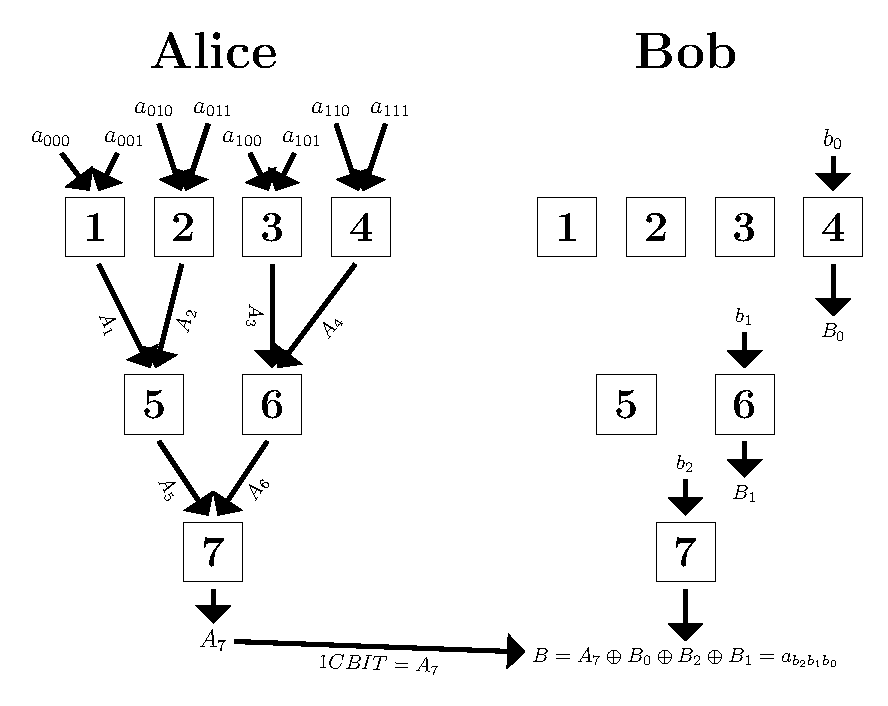
\includegraphics[scale=0.6]{1.eps}
\caption{  The figure demonstrates the use of concatenation of $(2\rightarrow1)$ RB
to form a $(2^{3}\rightarrow 1)$ RB. \textit{RESOURCE: $2^{3}-1=7$ }$(2\rightarrow 1)$
RB. In the figure Bob is trying to learn $a_{101}$ or $a_{111}$.}
\end{figure}
\subsection*{Addition} 
Let us start with a no-signaling $(n\rightarrow 1)$ RB($1$) and a no-signaling $(m\rightarrow 1)$ RB($2$).
We aim at winning the $(n+m\rightarrow 1)$ RAC. The protocol to achieve that is
as follows, \\
\textit{For winning the $(n+m \rightarrow 1)$ box using a no-signaling $(n\rightarrow 1)$ RB, a no-signaling $(m\rightarrow 1)$ RB, an additional  no-signaling $(2\rightarrow 1)$ RB and 1 c-bit of communication:}
Alice has $n$ input bits $a_{0},a_{1}..a_{n-1}$ corresponding to the
no-signaling $(n\rightarrow 1)$ RB($1$) and $m$ inputs bits  $a_{n},a_{n+1}..a_{n+m-1}$
corresponding to the no-signaling $(m\rightarrow 1)$ RB($2$), in total $n+m$ input bits. Alice Obtains a
output bit $A_{1}$ from the no-signaling $(n\rightarrow 1)$ RB($1$) and $A_{2}$ from the no-signaling $(m\rightarrow 1)$
RB($2$).
The {cost} of addition is an additional no-signaling $(2\rightarrow 1)$ RB($3$) whose
input bits are $A_{1}$ and $A_{2}$ and output bit is $A_{3}$. Alice then sends $m=A_{3}$ 
On Bob's end, Bob receives $b\in\{0,1..n-1,n,..n+m-1\}$ and message
$m$. \\
If $0\leq b<n$ then Bob enters $0$ in the no-signaling $(2\rightarrow 1)$ RB(2) and
obtains $B_{3}$ and enters $b$ into no-signaling $(n\rightarrow 1)$ RB($1$) to get
$B_{1}$ and outputs $B=m\oplus B_{1}\oplus B_{3}=a_{b}$.
If $n\leq b\leq n+m-1$ then Bob enters $1$ in the no-signaling $(2\rightarrow1)$ RB(2)
and obtains $B_{3}$ and enters $b$ into no-signaling $(m\rightarrow 1)$ RB($2$) to
get $B_{2}$ and outputs $B=m\oplus B_{2}\oplus B_{3}=a_{b}$.\\
For example winning $(m+n\rightarrow 1)$ RAC using no-signaling $(m\rightarrow 1)$ RB, no-signaling $(n\rightarrow1)$ RB and
a $(2\rightarrow1)$ RB [see FIG. 2].

\begin{figure} 
\includegraphics[scale=0.325]{ADD.pdf}
\caption{  The figure demonstrates the use of addition $(m\rightarrow1)$ RB, $(n\rightarrow 1)$ RB using
a no-signaling $(2\rightarrow1)$ RB.
RB. In the figure Bob is trying to learn $a_b$ for $n\leq b\leq n+m-1$.}
\end{figure}
Finally, protocol for winning the $(n\rightarrow 1)$ RAC using only the no-signaling $(2\rightarrow 1)$ RBs for any $n\in N$. \\
\textit{Protocol for  winning $(n\rightarrow1)$ RAC using no-signaling $(2\rightarrow1)$ RBs:} Any Natural number $n$ can be broken into sum of some discrete powers of $2$, i.e. $n=\sum_{i=0}^{k-1}\alpha_i2^i$ where $\alpha_i\in \{0,1\}$, $i\in\{0,k-2\}$ and $\alpha_{k-1}=1$, $k\in N$ such that $2^{k-1}\leq n< 2^k$. The coefficients $(\alpha_0\alpha_1..\alpha_{k-1})_2$ form the binary representation. We use a variable $count\in N$ and initialize it to $count=0$ for cost calculation given later. Alice receives $n$ input bits and for $i\in \{0,k-1\}$ such that when $\alpha_i=1$, she repeats the following steps,
\begin{enumerate}
\item Use concatenation of $2^i-1$ no-signaling $(2\rightarrow 1)$ RB to construct a $(2^i\rightarrow 1)$ RAC for $i>0$ and for $i=0$ simply take the first input bit $a_0$. Update $count=count+1$ and RB(RIGHT)=$2^i\rightarrow 1$ RB.
\item If $count=1$ Let RB(LEFT)= RB(RIGHT).
\item  If $count>1$: use a no-signaling $(2\rightarrow1)$ RB and ADDTION of $(x\rightarrow1)$ RB(LEFT) and $(y\rightarrow1)$ RB(RIGHT) to form the updated $(x+y\rightarrow 1)$ RB(LEFT).
\end{enumerate}
Alice sends the output of final (bottom most) $(2\rightarrow1)$ RB as the message bit $m$.
Bob receives the message bit $m$ and $b\in\{0,1,2,..,n-1\}$ and outputs $B=a_b$ by following corresponding parts of concatenation and addition. \\
\textit{Cost}: The variable count stores the total number of indexes $i$ such that $_i=1$. concatenation repeated count times uses $(n-count)$ no-signaling $(2\rightarrow1)$ RB. addition is repeated $(count-1)$ each time costing $1$ no-signaling $(2\rightarrow1)$ RB. Finally total cost is $(n-count)+(count-1)=n-1$ no-signaling $(2\rightarrow1)$ RB.
For example winning $(7\rightarrow 1)$ RAC using $(6)$ $(2\rightarrow 1)$ RB [see FIG. 6].
It is to be noted at this point that the protocol given above is just one of many possibilities for simulation of $(n\rightarrow 1)$ RAC using $(n-1)$ $(2\rightarrow 1)$ RB. In particular any construction which forms a fully connected binary tree with no-signaling $(2\rightarrow 1)$ RB as nodes can be used for the simulation $(n\rightarrow 1)$ RAC. In Appendix B we give the proof that $(n-2)$ $(2\rightarrow 1)$ RB (or equivalently PR) cannot simulate $(n\rightarrow 1)$ RAC.  

\textit{Classical and quantum winning probability of $(n\rightarrow1)$ RAC using the above protocol and corresponding bounds on $(2\rightarrow1)$} RAC.\\
One can win the $(n\rightarrow1)$ RAC using $n-1$ no-signaling $(2\rightarrow1)$ RB. Let the quantum and classical winning probabilities over the $(n\rightarrow1)$ RAC be $T_n$ and $C_n$. As the protocol above requires no-signaling $(2\rightarrow1)$ RBs, and  $T_2=\frac{2+\sqrt[]{2}}{4}$ and $C_2=\frac{3}{4}$ are enough to determine $C_n$ and $T_n$ for all $n\in N$ \cite{pawlowski2009information}. Let the winning probability of $(2\rightarrow1)$ RAC be $0<p_2<1$. As an example for $(7\rightarrow1)$ RAC [see FIG. 3] the probability that Bob guesses $a_b$ correctly is $p(B=a_b|b=0)=p_2^2+(1-P^2)^2$,$p(B=a_b|b=1)=(p_2^2+(1-p_2)^2)(p_2)+(1-p_2^2-(1-p_2)^2)(1-p_2)$ and $p(B=a_b|b\in \{1,2,3,4,5,6\})=p(B=a_b|b=1)$. Now Bob's inputs are uniformly distributed, hence $p_7=p(B=a_b)=\frac{p(B=a_b|b=0)+6p(B=a_b|b=1)}{7}$,  $T_7=0.68723$. Similarly, for $(n\rightarrow1)$ RAC for $n\in \{2,..10\}$ the protocol, $C_n$ and $T_n$ are provided in [see FIG. 6]. While $C_n$ are not optimal for $n=2k+1$ \footnote{majority function is not taken into account.}, $T_n$ are numerically close to known optimal values.
\begin{figure*} 
\includegraphics[scale=0.3]{Protocol.pdf}
\caption{ \label{boundMeToTheGround} (Color online)  The figure demonstrates the use of protocol described in Appendix C and $n-1$ no-signaling $(2\rightarrow1)$ RB to win the $(n\rightarrow1)$ RAC for $n\in \{2,3,..10\}$. The C and Q bounds, $C_n$ and $T_n$ are derived recursively using $C_2=0.75$ and $T_2=\frac{2+\sqrt[]{2}}{4}$.  }
\end{figure*}


\section*{Appendix D}
Here we provide the proof for resource inequality in Theorem 5 and consequently the in-equivalence of no-signaling $(2\rightarrow 1,3)$ RB\textsuperscript{2} and $B^3_2$. We give the proof in two parts: 
\begin{enumerate}
\item We shall show that if the $3$it of communication is not used to send the output of Alice's RB $A$ but $B^3_2$-box is obtained, then the channel $\Lambda_3$ is a depolarizing channel: it outputs $z$  or a random $3$it with $\frac{1}{2}$ probability.
\item If the $3$it of communication is used to send $A$ and $B^3_2$-box is obtained, then the capacity of obtainable channel $\Lambda_3$ is upper bounded by $\frac{1}{2}$ $3$it. 
\end{enumerate}
\subsection*{Proof part 1.}
Let $m$ be the message $3$it to be sent to Bob. The goal is to obtain  $B^3_2$-box i.e. $Y=x_y-_3X$ in any case $m=0,1,2$. In general for any $m$ Bob's output is a function of his input $y$ along with the RB $Y=Y(y,b,B)$. Now there are two cases:
\begin{enumerate}
\item \textbf{$A=A'$}: In this case the $B^3_2$-box is obtained by processing a perfect $(2\rightarrow 1,3)$ RAC.
\item \textbf{$A\neq A'$}: In this case the no-signaling $(2\rightarrow 1,3)$ RB\textsuperscript{2} outputs $B$ which does not depend on the work of RAC and hence is useless. Hence Bob's outcome only depends on the input he receives i.e. $Y=Y(y)$. Now we need for  $B^3_2$-box, $Y(y=0)=-_3X$ as $x_0=0$ and $Y(y=1)=x_1-_3X$. Notice Bob can compute $x_1$ using the fact $Y(y=1)-_3Y(y=0)=x_1$. Therefore in this case Bob must know the value of $x_1$.  
\end{enumerate}
Therefore $p_g(x_1|m=m_0)=1$ or $p_g(A|m=m_0)=1$ or both. Where $p_g$ denotes Bob's guessing probability. W.l.o.g. we assume that all three values of $m$ occur with non-zero probability. Bob's simplest strategy (of guessing only one variable, $x_1$ or $A$ for given $m$) can rely on 8 different cases:
\begin{enumerate}
\item $p_g(A|m=0)=1$,$p_g(A|m=1)=1$ and $p_g(A|m=2)=1$
\item $p_g(x_1|m=0)=1$,$p_g(x_1|m=1)=1$ and $p_g(x_1|m=2)=1$
\item $p_g(A|m=0)=1$,$p_g(A|m=1)=1$ and $p_g(x_1|m=2)=1$
\item $p_g(A|m=0)=1$,$p_g(x_1|m=1)=1$ and $p_g(A|m=2)=1$
\item $p_g(x_1|m=0)=1$,$p_g(A|m=1)=1$ and $p_g(A|m=2)=1$
\item $p_g(x_1|m=0)=1$,$p_g(x_1|m=1)=1$ and $p_g(A|m=2)=1$
\item $p_g(x_1|m=0)=1$,$p_g(A|m=1)=1$ and $p_g(x_1|m=2)=1$
\item $p_g(A|m=0)=1$,$p_g(x_1|m=1)=1$ and $p_g(x_1|m=2)=1$
\end{enumerate}
In the third case (equivalently for fourth to eighth cases) Bob makes a perfect guess of $A$ for $m=0,1$ and of $x_1$ for $m=2$. We shall now show by an example (others are analogous), that for the conditions in the third case such a joint probability distribution $p(A,x_1,m)$ cannot exist. Suppose Bob makes a perfect guess, e.g. $A=0$ for $m=0$, $A=1$ for $m=1$ and $x_1=0$. We find that $p(A=2,x_1=1)=0$ and $p(A=2,x_1=2)=0$, which implies the reduced probability distribution $p(A,x_1)$ is no longer randomly distributed, but RB works in a way such that $A$ and $x_1$ are generated independently at random.\\
From the only two possible cases we see that in the first case, $m$ is simply used to send $A$. This case is further dealt with in the Part 2. In the second case the message bit is used to send $x_1$ in this $B^3_2$ box is obtained and the RB serves as an depolarizing $3$it channel with probability $\frac{1}{2}$. $\blacksquare$ 
\subsection*{Proof part 2}
We shall use information theoretic tools to show that if the no-signaling $(2\rightarrow 1,3)$ RB\textsuperscript{2} supplemented with one bit of communication is able to reproduce exactly the $B^3_2$-box and some $3$it channel, then the mutual information of that channel must be bounded by $\frac{1}{2}$ (assuming that Alice's output of RB $A$ is directly inserted into Bob input to the RB i.e. $A=A'$). \\
We shall use the following common assumptions:\\
\textit{Assumptions:} Alice is supplied with two $3$its $x_1,z$, Bob is given a bit $y$. Both are given access to shared random $3$it $s$ such that $x_1,z,y,s$ are mutually independent. Alice generates $X$ and inputs for the RB $a_0,a_1$ from $x_1,z,s$. Similarly Bob generates his input to the RB $b$ from $y,s$. These strategies result in shared joint probability distribution $p(x_1,z,y,s,b,B,X,Y)$ such that $B=a_b$ is obtained from the RAC on Bob's side (as $A$ is always inserted into $A'$) , and $Y$ is generated out of $b,B,s,y$. 
We shall first reformulate Theorem 5 in other words.
Under the aforementioned assumptions, if variables $x_1,y,X,Y$ perfectly reproduce the $B^3_2$-box, there holds:
\begin{equation}\label{main}
I(z:B,b,y,s)\leq \frac{1}{2}
\end{equation}

We shall prove this Theorem in two parts:
\begin{enumerate}
\item First we shall use entropies and correlation to state the fact that to simulate the $B^3_2$-box Bob has to guess perfectly $X$ when $y=0$ and $x_1-_3X$ when $y=1$. 
\item Second we shall show that it is impossible to send more than 1 $3$it through a channel with 1 $3$it capacity. As in our case Alice would like to send both $x_1$ and $z$ which bounds Bob's possible information gain about $z$. 
\end{enumerate}
\begin{mydef2}
Under the aforementioned assumptions, if variables $(x_1,y,X,Y)$ simulate the $B^3_2$-box, there holds:
\begin{eqnarray} \label{ae1}
I(B:x_1-_3X|b,s,y=1)=\nonumber \\H(x_1-_3X|b,s,y=1) \\ \label{ae2}
I(B:X|b,s,y=0)=\nonumber \\ H(X|b,s,y=0) 
\end{eqnarray}
\end{mydef2}
Now in order to perfectly reproduce $B^3_2$-box given $y=0$, he should perfectly guess $X$. On the other hand, given $y=1$ he should perfectly guess $x_1-_3X$. So we must have:
\begin{equation}
J(B,b,s,y=0\rightarrow X)=1 
\end{equation}
and
\begin{equation}
J(B,b,s,y=1\rightarrow x_1-_3X=1 
\end{equation}
where $J(\mathcal{X} \rightarrow \mathcal{Y})=\Sigma_ip(\mathcal{X}=i)\max_j[p(\mathcal{Y}=j|\mathcal{X}=i)]$. Which implies that there must be $max_j[p(X=j|B=l,b=l,y=0,s=i)]=1$, and consequently $H(X|B,b,y=0,s)=0$ which directly leads to (\ref{ae1}). Analogously for (\ref{ae2}). $\blacksquare$\\
\textit{One cannot send more than one $3$it through a single $3$it wire}\\
Here we prove the main argument of Theorem 5. That is, the following Theorem shows the tradeoff between Bob's correlations with $X$ and $x_1-_3X$ and his correlations with $z$. 
\begin{mydef1} \label{At2}
Under aforementioned assumptions, there holds:
\begin{eqnarray} \label{pe1}
\frac{1}{2}I(x_1-_3X:B|b,s,y=1)+\nonumber \\ \frac{1}{2}I(X:B|b,s,y=1)+I(z:B|b,s,y) \leq \nonumber \\ 
\frac{1}{2}I(X:x_1-_3X:z|b,s)+H(B|b,s,y)
\end{eqnarray}
\end{mydef1}
To prove this Theorem we use the following fact:
\begin{eqnarray} \label{te3}
I(S:T|V)+I(T:U|V) \leq 
I(S:U|V)+\nonumber \\ I(T:SU|V)  \equiv I(S:T:U|V)
\end{eqnarray}
The LHS of (\ref{te3}) can be reformulated as, upon fixing $s=i$:
\begin{eqnarray}
\frac{1}{2}I(x_1-_3X:B|b,s=i,y=1)+\nonumber \\ \frac{1}{2}I(X:B|b,s=i,y=1)+I(z:B|b,s=i,y=0) \nonumber \\ I(z:B|b,s=i,y=1)
\end{eqnarray}
Now using (\ref{te3}) to first and third terms and to second and fourth terms, we find that the above quantity is upper bounded by,
\begin{multline}
\frac{1}{2}[I(x_1-_3X:z|b,s=i,y=1)+ \\ I(B:x_1-_3,z|b,s=i,y=1)+ \\ I(X:z|b,s=i,y=0) + \\ I(B:X,z|b,s=i,y=0)]
\end{multline}
Now as $(x_1-_3X,z|s=i)$ is independent from $(y,b|s=i)$, therefore $I(x_1-_3X:z|b,s=i,y=1)=I(x_1-_3X:z|b,s=i)$. And since $(X,z|s=i)$ is independent from $(y,b|s=i)$, there is $I(X:z|b,s=i,y=0)=I(X:z|b,s=i)$. Multiplying these with $p(s=i)$ and summing over values of $s$ we obtain:
\begin{multline}
\frac{1}{2}[I(x_1-_3X:z|b,s)+ \\ I(B:x_1-_3X,z|b,s,y=1)+ \\ I(X:z|b,s) + \\ I(B:X,z|b,s,y=0)]
\end{multline}
We can now use (\ref{te3}) to the first and third terms to obtain the upper bound:
\begin{multline}
\frac{1}{2}[I(x_1-_3X:X|b,s)+ \\ I(z:X,x_1-_3X|b,s)+ \\ I(B:x_1-_3X,z|b,s,y=1) + \\ I(B:X,z|b,s,y=0)]
\end{multline}
Now $I(x_1-_3X:X|b,s)+I(z:X,x_1-_3X|b,s)=I(z:X:x_1-_3X|b,s)$. Also 
$\frac{1}{2}[I(B:x_1-_3X,z|b,s,y=1) +  I(B:X,z|b,s,y=0)]\leq H(B|b,s,y)$, and (\ref{pe1}) follows. $\blacksquare$\\
Finally, we shall proof the inequality (\ref{main}). From the chain rule: $I(z:B,b,s,y)=I(z:y,s,b)+I(z:B|y,s,b)$ but $I(z:y,s)=I(z:y,b,s)=0$ ($b=b(y,s)$). Hence \ref{main} can be reformulated as:
\begin{equation} \label{main2}
I(z:B|s,b,y)\leq \frac{1}{2}
\end{equation}
To prove (\ref{main2}) we shall reformulate (\ref{pe1}) using (\ref{ae1}) and (\ref{ae2}):
\begin{multline}
\frac{1}{2}[H(X|b,s,y=0)+H(x_1-_3X|b,s,y=1)]+\\I(z:B|b,s,y) \leq \frac{1}{2}[H(X|b,s)+H(x_1-_3X|b,s)+\\H(z|b,s)-H(X,x_1-_3X,z|b,s)]+\\H(B|b,s,y)
\end{multline}
Now as $(X|s=i)$  and $(x_1-_3X|s=i)$ are independent from $(b,y|s=i)$, we have for each $i$ that $H(X|b,s=i,y=0)=H(X|b,s=i)$ and $H(x_1-_3X|b,s=i,y=1)=H(x_1-_3X|b,s=i)$. And because for some fixed $s=i$, $z$ is independent of $b$, we have $H(z|b,s=i)=H(z|s=i)$. Averaging these equalities over $p(s=i)$ we obtain:
\begin{multline}
I(z:B|y,b,s) \leq \\ \frac{1}{2}[H(z|s)-H(X,x_1-_3X,z|b,s)]+H(B|y,s,b)
\end{multline}
Now $z$ is independent of from $s$, $H(z|s)=H(z|s)=1$. And $H(X,x_1-_3X,z|s)=H(X,x_1,z|b,s)$ as we can add $X$ to $x_1-_3X$. Using the data processing inequality and the independence of $s$ form $(x,z)$ we get, $H(z,X,x_1|s)\geq H(z,x_1|s)=H(z,x_1)=2$. Hence the first two terms are upper bounded by $-\frac{1}{2}$. The last term trivially upper bounded by $1$, which results in $\frac{1}{2}$ proving (\ref{main2}) $\blacksquare$.

\end{document} 
